\chapter{机械通气与撤机}

\section{前沿学术综述}

急性呼吸衰竭是以低氧血症为特征的急性起病的呼吸衰竭,是威胁危重病人生命的常见危重症。20世纪50年代以来,机械通气逐渐成为急性呼吸衰竭最重要的支持治疗手段。

\subsubsection{机械通气的生理与临床目标}

机械通气的临床应用中,往往存在两个突出问题,一是过分强调机械通气的指征,而有关指征又局限于呼吸生理指标,对于危重病人来说,难以确定恰当的机械通气时机,使不少患者痛失早期治疗的有利时机,这在严重急性呼吸综合征(SARS)呼吸衰竭的处理上表现得尤为突出;二是机械通气的目的不明确,导致治疗缺乏个体化,使机械通气未能获得积极的疗效。因此,合理的机械通气首先必须明确机械通气的目标。明确有创机械通气的生理和临床目标,既有助于解决指征问题,以免延误治疗,同时又能使机械通气治疗实现个体化,获得最佳疗效。机械通气的生理目标主要包括
\protect\hyperlink{text00016.htmlux5cux23ch1-15}{\textsuperscript{{[}1{]}}}
\textsuperscript{,}
\protect\hyperlink{text00016.htmlux5cux23ch2-15}{\textsuperscript{{[}2{]}}}
:

(1)改善或维持动脉氧合 改善低氧血症,提高氧输送是机械通气最重要的生理目标。吸入氧浓度适当条件下,动脉血氧饱和度>90%或动脉氧分压>60mmHg(1mmHg=0.133kPa)是保证氧输送的前提。由于组织氧输送是由动脉血氧饱和度(或动脉血氧分压)、血红蛋白浓度和心输出量共同决定,过分强调动脉氧分压达到正常水平对机体并无益处。

(2)支持肺泡通气 使肺泡通气量达到正常水平,将动脉二氧化碳分压水平维持在基本正常的范围内,是机械通气的基本生理目标之一。但对于颅内高压患者,往往需要提高肺泡通气量,使动脉二氧化碳分压低于正常以降低颅内压;对于ARDS患者,由于肺泡容积明显减少,为防止呼吸机相关性肺损伤,需采用小潮气量,允许动脉二氧化碳分压有所升高。

(3)维持或增加肺容积 维持或增加肺容积是机械通气中常被忽视的生理目标。肺泡容积明显减少主要见于肺不张、ARDS、肺部感染、肺水肿等,是患者出现呼吸窘迫、低氧血症和肺顺应性明显降低的主要原因。通过应用控制性肺膨胀、间歇性高水平呼气末正压(PEEP)、叹息、俯卧位通气等肺泡复张手段,可明显增加呼气末肺泡容积(功能残气量),改善呼吸窘迫和低氧血症。

(4)减少呼吸功 机械通气替代患者呼吸肌肉做功,降低呼吸肌氧耗,有助于改善其他重要器官或组织的氧供。正常情况下,呼吸肌氧需占全身氧需的1%~3%,呼吸困难或呼吸窘迫时,氧需骤增,使得氧需增加到全身氧需的20%~50%。呼吸氧需的明显增加,势必造成其他器官的缺氧,可能导致或加重多器官功能障碍综合征(MODS),上消化道出血常常是发生MODS的先兆。及时的机械通气治疗,改善呼吸困难,能明显降低呼吸肌氧需,防止MODS。

强调机械通气的生理目标无疑是很重要的,但机械通气的临床目标对机械通气的指导更直接、更具可操作性。临床目标主要包括:①纠正低氧血症,通过改善肺泡通气量、增加功能残气量、降低氧耗,可纠正低氧血症和组织缺氧;②纠正急性呼吸性酸中毒,但动脉二氧化碳分压并非一定要降至正常水平;③缓解呼吸窘迫,缓解缺氧和二氧化碳潴留引起的呼吸窘迫;④防止或改善肺不张;⑤防止或改善呼吸肌疲劳;⑥保证镇静剂和肌松剂使用的安全性;⑦减少全身和心肌氧耗;⑧降低颅内压,通过控制性的过度通气,降低颅内压;⑨促进胸壁的稳定,胸壁完整性受损的情况下,机械通气可促进胸壁稳定,维持通气和肺膨胀
\protect\hyperlink{text00016.htmlux5cux23ch1-15}{\textsuperscript{{[}1{]}}}
\textsuperscript{,}
\protect\hyperlink{text00016.htmlux5cux23ch2-15}{\textsuperscript{{[}2{]}}}
。

\subsubsection{机械通气实施中遵循的原则}

(1)个体化原则 不同疾病和不同病程,机械通气的设置应有所不同。随病情改变,也需随时调整机械通气的支持条件。重度ARDS肺容积明显降低,需要采用小潮气量,即允许性高碳酸血症。对于轻度ARDS患者,肺容积接近正常,可采用接近正常的潮气量
\protect\hyperlink{text00016.htmlux5cux23ch3-15}{\textsuperscript{{[}3{]}}}
。

(2)氧输送原则 机械通气的根本目的是保证全身氧输送,改善组织缺氧。因此,单纯强调提高动脉氧分压是片面的。过高的通气条件干扰循环,使动脉氧分压的提高以心排出量下降为代价,则降低氧输送,加重组织缺氧,将使呼吸治疗得不偿失。血流动力学监测及氧输送监测对机械通气的重症患者是非常必要的。

(3)肺保护原则 机械通气不当可引起呼吸机相关性肺损伤等严重并发症,不但可加重肺损伤,而且也可导致正常肺组织损伤。因此,机械通气时坚持肺保护原则就显得很重要。不应把正常生理指标作为机械通气的目标,如ARDS肺容积明显减少,应采取允许性高碳酸血症的通气策略,为防止肺泡跨壁压过高,应保证气道平台压力低于35cm
H\textsubscript{2} O(1cm H\textsubscript{2}
O=0.098kPa),防止呼吸机相关性肺损伤
\protect\hyperlink{text00016.htmlux5cux23ch4-15}{\textsuperscript{{[}4{]}}}
。

(4)动态监测原则 机械通气过程中,应动态监测潮气量、气道压力、呼吸频率、分钟通气量、PEEP及内源性PEEP等呼吸生理参数。气体闭陷或内源性PEEP导致的动态肺过度充气常见于哮喘、慢支等气道阻塞患者,常被忽视。监测内源性PEEP,才有可能及时发现和防止动态肺过度充气,避免其不良影响。监测上述参数的同时,应监测经皮血氧饱和度(SpO\textsubscript{2}
)、呼气末二氧化碳等,确保机械通气能够有效的改善通气和换气功能。

(5)MODS防治原则 机械通气不当不但可加重肺损伤,而且可引起或加重肺外的多器官功能衰竭(即MODS)。以往认为,机械通气对肺外器官的影响主要与循环干扰有关。一般情况下,机械通气对循环功能的影响不明显,但对于血容量明显不足或休克的患者,正压通气对循环具有一定抑制作用。表现为静脉回心血量减少和心输出量降低,导致循环更不稳定和肠道等内脏器官灌注降低。当然,影响程度与机械通气条件和患者代偿能力等因素有关
\protect\hyperlink{text00016.htmlux5cux23ch2-15}{\textsuperscript{{[}2{]}}}
。

近年来,ARDS机械通气研究结果令人瞩目,使机械通气对急性呼吸衰竭的治疗影响从肺部扩展到全身各器官,特别是注意到不适当的机械通气激活和放大肺部炎症反应,并导致炎症介质向循环系统移位,可能导致或加重MODS。10年前我们就注意到,仅有13%的ARDS死于呼吸衰竭,而绝大多数患者死于肺外器官衰竭或MODS,但机制不清楚。目前基本证实,以大潮气量和低PEEP为特征的传统机械通气策略,不但明显加重ARDS肺部炎症反应,而且可导致正常肺组织中炎症细胞激活和炎症介质释放,肺泡和间质中炎症介质和毒素向毛细血管移位,介导或加重MODS
\protect\hyperlink{text00016.htmlux5cux23ch5-15}{\textsuperscript{{[}5{]}}}
。可见,不合理的机械通气治疗可使ARDS向MODS发展,增加ARDS病死率,这一认识是近10年来急性呼吸衰竭机械通气治疗的最显著的进步。

更令人兴奋的是,最近美国国立卫生研究所(NIH)组织的多中心随机研究显示,与传统大潮气量(11.8ml/kg)比较,小潮气量(6.2ml/kg)+最佳PEEP明显缩短ARDS患者机械通气时间,而且病死率显著降低(分别为39.8%和31.0%)
\protect\hyperlink{text00016.htmlux5cux23ch6-15}{\textsuperscript{{[}6{]}}}
。Villar的研究进一步证实了肺保护性通气可降低ARDS的病死率
\protect\hyperlink{text00016.htmlux5cux23ch5-15}{\textsuperscript{{[}5{]}}}
。这一结果标志着ARDS治疗策略的根本性突破。应用小潮气量+最佳PEEP为主要内容的肺保护性通气策略,不仅是重要的肺支持性治疗措施,也成为ARDS病因性治疗及MODS防治的重要手段。可见,采用适当的机械通气策略,防止呼吸机相关性肺损伤及其介导的全身炎症反应,进而防止MODS,是机械通气实施中必须重视的问题。

\subsubsection{机械通气模式选择}

(1)压力控制与容量控制的选择 容量控制通气和压力控制通气都是常用的控制通气模式,均为时间切换。潮气量稳定,但也有局限性:①恒速气流,吸气早期的流速不足,使患者感觉“空气饥饿”,需额外做功,自主呼吸较强的患者尤为突出;②控制通气,清醒患者常不耐受,需镇静剂使患者与呼吸机同步;③气道阻力升高或胸肺顺应性降低时,气道峰值压力和平台压力升高,易导致气压伤。

压力控制通气采用减速气流,较符合生理需要,降低吸气早期的呼吸功,同时吸气早期流速较高,有助于使塌陷肺泡复张。气道压力能够限制在一定范围,减少气压伤发生。但压力控制通气潮气量不稳定,潮气量不仅与压力控制通气压力有关,还与胸肺顺应性和气道阻力有关,应用压力控制通气时应持续监测潮气量。对于气道阻力和顺应性不稳定的患者,宜采用控制通气;而对于吸气流速要求较高的患者,以及容易发生气压伤,需要限制气道压力的患者(如ARDS),应采用压力控制通气。

(2)反比通气中压力和容量控制模式的选择 生理状态时,吸气时间较呼气时间长,通常吸呼比为1∶1.5~1∶3。反比通气是延长吸气时间的一种通气方式,吸气时间较呼气时间长,通常吸呼比为1~2∶1,最高可达4∶1。反比通气通过延长吸气时间,提高平均气道压力,促进肺泡复张,同时呼气时间缩短,产生内源性PEEP,有利于增加功能残气量,改善低氧血症。

反比通气包括压力控制反比通气和容量控制反比通气。治疗严重低氧血症的急性呼吸衰竭时是否应采用反比通气,以及应采用压力控制反比通气还是容量控制反比通气,一直存在争议。以往认为压力控制反比通气优于容量控制反比通气,可避免气道峰值压过高而防止气压伤,同时吸气时间延长而产生内源性PEEP,明显改善氧合。但临床和实验研究显示,与传统的控制通气或压力控制通气相比,压力控制反比通气明显改善ARDS低氧血症。但若测定内源性PEEP,调整外源性PEEP,使总PEEP水平和潮气量等相同时,压力控制反比通气/容量控制反比通气与压力控制通气或容量控制通气在改善氧合方面并无明显优势,而且压力控制反比通气与容量控制反比通气也无明显差异。以往研究中反比通气改善氧合优于正比通气,可能与反比通气导致内源性PEEP,加上外源性PEEP,使总PEEP水平提高有关。如未监测内源性PEEP,则造成反比通气改善氧合的假象。说明反比通气改善氧合并不优于正比通气,其关键在于总PEEP水平是否适当。

(3)气道双相正压通气 气道双相正压通气是一种定时改变持续气道内正压水平的系统,呼吸机按照预设的两种不同压力水平进行通气。气道压力在高压与低压之间周期性地转换,存在自主呼吸的患者,自主呼吸可在双压力水平上进行
\protect\hyperlink{text00016.htmlux5cux23ch7-15}{\textsuperscript{{[}7{]}}}
。

气道双相正压通气包括了从压力控制通气到自主呼吸或持续气道内正压通气各种不同辅助程度的通气模式。无自主呼吸时,气道双相正压通气实际上就是压力控制通气,如果高压时间比低压时间长,则为压力控制反比通气;有自主呼吸时,自主呼吸可在高、低压两个水平上进行,其中高压水平的自主呼吸相当于持续气道内正压通气,当设置压力支持通气时,在低压水平上按压力支持通气的压力水平给予支持,保持了自主呼吸,减少了人机对抗。当高压与低压水平相同时,即持续气道内正压通气。

与容量控制反比通气比较,气道双相正压通气能够更好的改善氧合和肺内分流,而且具有较低的平均气道压力,全身氧输送略有升高。

气道双相正压通气具有明显的优势:①平均气道压力低,防止气压伤;②保持不同水平的持续气道内正压通气,可有效促进塌陷肺泡复张,改善氧合;③双相压力和时间可随意调整,包括了不同辅助程度的通气模式,使用范围广;④通气系统完全开放,高压与低压水平均可进行自主呼吸,循环干扰小,而且人机对抗少,有利于呼吸肌功能锻炼和撤机。目前认为气道双相正压通气是实施肺保护性通气的最佳模式之一。

\subsubsection{机械通气的参数设置}

(1)PEEP的设置 PEEP通过呼气末肺泡内正压的支撑作用防止肺泡塌陷,改善气体交换。其效应与PEEP水平密切相关。最佳PEEP可以消除塌陷肺泡反复复张产生的剪切力,减轻肺损伤,同时增加功能残气量,改善通气/血流比例,从而改善低氧血症。

选择最佳PEEP,既可防止呼气末肺泡萎陷,又能避免肺泡过度膨胀。静态压力-容积曲线低位转折点法和最大氧输送法是ARDS选择最佳PEEP常用的临床方法,但实用性均较差。最近应用低流速法(<8L/分钟)测定动态肺压力-容积曲线,获得准静态压力-容积曲线,与静态压力-容积曲线高度相关,使床边选择最佳PEEP成为可能。一般以高于准静态压力-容积曲线低位转折点压力2~3cm
H\textsubscript{2}
O作为最佳PEEP。对于胸部或上腹部手术患者,术后采用3~5cm
H\textsubscript{2} O的PEEP,有助于防止肺不张和低氧血症。

(2)潮气量设置 容量控制通气时,潮气量设置的目标是保证足够的通气,并使患者较为舒适。成人潮气量一般为8~12ml/kg。应考虑胸肺顺应性、气道阻力、氧合状态、通气功能和发生气压伤的危险性。气压伤等呼吸机相关性肺损伤与潮气量过大或气道压力过高有关。设置潮气量一般要求气道平台压力不超过30~35cm
H\textsubscript{2} O。

(3)压力上升时间的调整 以往应用压力支持通气或压力控制通气时,吸气压力上升速度不能根据患者需要进行调整。近年来,一些新型呼吸机能够对吸气压力上升时间进行调整。一般来说,压力上升时间越短,呼吸机提供的气流流速越大。研究显示,压力上升时间越短,吸气峰值流速越大,明显降低呼吸功。与长压力上升时间(40%吸气时间)比较,采用最短压力上升时间时,压力支持通气5和15cm
H\textsubscript{2}
O的吸气做功分别降低23%和38%,但对潮气量和呼吸频率无明显影响。对慢性阻塞性肺疾病急性发作患者,较短的吸气压力上升时间同样能明显降低吸气做功。因此,若需进一步降低呼吸功,可将吸气压力上升时间缩短。

(4)呼气灵敏度 呼气灵敏度是吸气向呼气切换的灵敏度。一般认为,当呼吸机管道有微量漏气时,将呼气灵敏度调高可防止吸气过长。与40%峰值流速的呼气灵敏度比较,5%峰值流速呼气灵敏度时吸气时间明显延长,呼吸频率降低,潮气量增加,但呼吸功和吸气峰值流速无明显变化。因此,对于需降低呼吸频率、增加潮气量的患者,可适当降低呼气灵敏度,而需减少吸气时间的患者,可适当提高呼气灵敏度。

(5)气管插管补偿 辅助通气时,患者不但需克服自身负荷做功,还需克服气管插管及呼吸机等器械阻力而额外做功,即附加功。附加功使总呼吸功明显增加,患者易出现呼吸频速等脱机困难假象。气管插管补偿理论上能够完全克服气管插管的附加阻力,使患者只需克服自身的呼吸负荷。气管插管补偿对附加功的降低程度是其效率的主要决定因素
\protect\hyperlink{text00016.htmlux5cux23ch7-15}{\textsuperscript{{[}7{]}}}
。近来的研究表明,呼吸机补偿比例100%前提下,气管插管附加阻力的补偿并不能达到100%。一般情况下,气管插管补偿只能补偿50%~68%的吸气附加阻力,1%~26%的呼气附加阻力。虽然气管插管补偿能够一定程度的降低附加阻力,但不能完全补偿,需对其客观评价。

\section{临床问题}

\subsection{机械通气的指征与对器官功能的影响}

\subsubsection{出现哪些情况应考虑开始机械通气治疗?}

在出现较为严重的呼吸功能障碍时,应考虑机械通气。如果实施机械通气过晚,患者会因严重低氧和二氧化碳潴留而出现多脏器功能受损,此时机械通气的疗效显著降低。因此,机械通气宜早实施。符合下述条件应实施机械通气:①经积极治疗后病情仍继续恶化;②意识障碍;③呼吸形式严重异常,如呼吸频率>35~40次/分钟或<6~8次/分钟,或呼吸节律异常,或自主呼吸微弱或消失;④血气分析提示严重通气和(或)氧合障碍:动脉血氧分压<50mmHg,尤其是充分氧疗后仍<50mmHg;⑤动脉血二氧化碳分压进行性升高;⑥pH动态下降。

从呼吸生理指标来看,符合以下任何1项时,即需开始机械通气治疗:①自主呼吸频率高于正常3倍或低于正常1/3;②潮气量低于正常1/3;③生理死腔通气量/潮气量高于60%;④肺活量低于10~15ml/kg;⑤动脉血二氧化碳分压高于50mmHg(慢性阻塞性肺病除外),并且有继续升高的趋势或出现精神症状;⑥动脉血氧分压低于正常的1/3,或肺泡动脉氧分压差>50mmHg(吸空气者)或>300mmHg(吸纯氧);⑦最大吸气负压低于25cm
H\textsubscript{2}
O。这些指标虽然是很重要的,但患者是否需要机械通气治疗,关键还要根据患者的病情结合医师的临床经验来综合判断。

\subsubsection{机械通气有哪些禁忌证?}

一般认为,机械通气没有绝对禁忌证,但有一些特殊疾病,应首先做必要的处理才能进行机械通气,或需采用特殊机械通气手段,否则可能会给患者带来不良影响。因此,对于这些特殊疾病,可归结为机械通气的相对禁忌证,以提醒临床医师采取适当的处理手段。这类疾病主要包括:

(1)张力性气胸或气胸 气胸患者接受机械通气治疗,易发生张力性气胸,而张力性气胸患者如接受机械通气治疗,则病情会进一步恶化。因此,这类患者在接受机械通气前或同时,必须采取胸腔闭式引流。

(2)大咯血或严重误吸引起的窒息性呼吸衰竭 大咯血或严重误吸引起的窒息,不宜立即用呼吸机进行正压通气,因为气道被血块或误吸物阻塞,正压通气会把血块或误吸物压入小支气管而易发生肺不张,对以后的治疗和恢复不利。应首先采取措施,将血块或误吸物清除,再进行正压通气。当然,不能一味地强调清除血块或误吸物而导致患者通气不足和缺氧,在清除误吸物的同时,应保证供氧。

(3)伴肺大疱的呼吸衰竭 肺大疱患者接受机械通气时,大疱内压力可升高而引起大疱破裂,引起张力性气胸。这类患者使用呼吸机时应注意患者肺大疱的程度、范围及是否有气胸病史,正压通气的压力应尽可能低,而且在机械通气过程中,应密切注意观察患者生命体征和肺部体征,以防发生气胸。一旦发生气胸,应立即进行胸腔闭式引流。

(4)严重心衰继发性的呼吸衰竭 目前认为严重心衰患者如并发呼吸衰竭,也应实施机械通气,但机械通气有可能影响心脏前后负荷,因此需要选择适当的机械通气模式,将机械通气对循环的影响降到最低限度,并密切观察循环的改变,必要时应持续监测血流动力学变化。

\subsubsection{机械通气对循环功能有何影响?}

机械通气对循环功能的影响程度与机械通气条件和患者代偿能力等多方面因素有关。机械通气对循环的影响主要取决于以下两个因素:

(1)胸内压力升高 机械通气使胸腔内压升高,导致静脉回流减少,心脏前负荷降低,其综合效应往往是心输出量降低,血压降低。血管容量相对不足或对前负荷较依赖的患者尤为突出。常在机械通气开始时、增加呼气末正压水平或延长吸气时间时出现血压降低,快速输液或通过调整通气模式降低胸腔内压,多能使低血压改善。另外,由于机械通气使患者胸腔内压力与胸腔外的压力差增大,导致心脏后负荷降低。对于某些充血性心衰患者,机械通气一方面可降低前负荷,同时又可降低后负荷,可见,机械通气有助于改善这类患者的心功能。

(2)肺血管阻力升高 当肺容积接近功能残气量时,肺血管阻力最低。肺容积高于功能残气量(见于肺过度膨胀)或低于功能残气量(见于肺萎陷),均可导致肺血管阻力增加。如采用通气模式适当,既可使塌陷的肺泡复张,又能避免肺泡过度膨胀,则可能使肺血管阻力降低;否则,可导致肺血管阻力增加、肺动脉压力升高、右室压力升高,影响右室功能,同时,由于左心室充盈不足,结果导致室间隔左偏,又损害左心室功能。对于存在肺动脉高压或右心室功能不全的患者,上述情况尤为突出。

\subsubsection{机械通气对重症患者肾功能有什么影响?}

缺氧可引起肾功能损害,经机械通气治疗,纠正缺氧后,肾功能损害可好转。但机械通气对肾脏功能有明显影响,主要表现为以下两方面:

(1)水钠潴留 机械通气引起患者胸腔内压力升高,使静脉回流减少,刺激心房的容量感受器,导致抗利尿激素释放增加,致肾脏集合管对水的重吸收增加,导致机体水钠潴留。

(2)肾脏灌注减少 机械通气导致静脉回流减少,使心脏前负荷降低,而肺血管阻力增加,又使右心后负荷增加,结果导致心排出量降低,导致肾脏血流灌注减少。

对于肾脏功能不全的患者或肾脏灌注已明显减少的患者,实施机械通气时,应注意机械通气的上述影响,避免肾脏功能的恶化。

\subsubsection{机械通气对中枢神经系统功能有何影响?}

机械通气主要通过影响动脉血二氧化碳分压和颈内静脉回流而影响中枢神经系统功能。脑动脉血管对动脉血二氧化碳敏感,当通气过度引起动脉血二氧化碳分压低于正常时,可引起脑动脉血管痉挛,使脑血流量减少。当动脉血二氧化碳分压低于20mmHg时,脑血流量可减少60%,因此,短时的过度通气使动脉血二氧化碳分压低于正常,有助于暂时性地改善脑水肿、降低颅内压,可作为颅高压患者的临时性应急治疗措施。当然,长时间过度通气,脑血流持续降低,可加重脑组织缺血缺氧,加重脑损伤。

当机械通气引起患者通气不足时,动脉血二氧化碳分压升高,结果可引起脑血管扩张,脑血流增加,可引起或加重脑水肿,使颅内压增高。

机械通气引起胸腔内压升高,特别是应用呼气末正压(PEEP)时,胸腔压力增加更为明显,可导致颈内静脉回流障碍,亦增加颅内压。因此,脑血管意外的患者及颅脑手术后的患者接受机械通气治疗时,应特别注意通气量和PEEP的调节。

\subsection{机械通气的参数设置和模式选择}

\subsubsection{重症患者接受机械通气应注意的基本问题有哪些?}

应用机械通气主要应注意以下原则:

(1)呼吸机条件的设置必须与病情相结合。不同疾病、不同病程,机械通气的模式和设置应有所不同,随病情改变,随时调整机械通气的支持条件。

(2)机械通气可引起多种并发症或不良影响,机械通气应用不当时尤为突出,因此,应采取相应措施,减少机械通气相关的并发症或不良影响。

(3)不应把正常生理指标作为机械通气的目标。一般把患者平素的呼吸状况作为机械通气的目标。对于ARDS患者为避免气压伤,甚至可允许动脉血二氧化碳分压高于正常,而不把动脉血二氧化碳分压接近正常水平作为机械通气的目标。

(4)肺泡过度膨胀、肺泡跨壁压过高是导致气压伤的重要原因,应采取措施防止肺泡跨壁压过高。一般认为,吸气末气道压力即平台压力,可作为估计肺泡跨壁压的临床指标,气道平台压>35cm
H\textsubscript{2}
O易导致气压伤,其肺损害程度远超过吸入高浓度氧。因此,避免气道平台压>35cm
H\textsubscript{2} O是十分必要的。

(5)气体闭陷或内源性呼气末正压(PEEP)等导致的动态肺过度充气常见于气道阻塞患者,但往往被忽视,临床必须关注这一问题,测定内源性PEEP,才有可能及时发现和防止动态肺过度充气,避免其不良影响。

(6)纠正低氧血症是机械通气的首要任务之一,但其根本目的是保证全身氧输送,改善组织缺氧。因此,单纯强调提高动脉氧分压是片面的,过高通气条件则干扰循环,使动脉氧分压的提高以心排出量下降为代价,继而降低氧输送,加重组织缺氧,使呼吸治疗得不偿失。肺动脉漂浮导管监测血流动力学及氧输送监测对机械通气的重症患者有时是非常必要的。

\subsubsection{重症患者接受机械通气治疗的主要准备工作和基本步骤有哪些?}

对于准备接受机械通气的患者,应按以下步骤作准备工作:

(1)首先明确患者是否具有机械通气的指征。

(2)如具有机械通气指征,那么就要判断患者是否具有机械通气的相对禁忌证并进行必要处理。

(3)根据病情确定患者需要控制呼吸或是辅助呼吸。对于呼吸完全停止或虽存在自主呼吸,但自主呼吸不能维持氧合者,应采用控制通气,主要包括容量控制通气和压力控制通气以及高频通气等;对于存在自主呼吸,但通气量不足或氧合部分障碍的患者,可采用辅助通气,视病情不同,可分别采用同步间歇指令通气、同步间歇指令通气+压力支持通气、容量支持通气、分钟指令通气、压力支持通气、持续气道内正压等。

(4)确定机械通气的每分通气量。一般情况下,按8~10ml/kg计算预设潮气量和每分通气量,动脉血二氧化碳分压维持在40mmHg左右。但每分通气量的设置应考虑到患者肺部疾病情况。严重ARDS患者,为防止气压伤,应降低每分通气量,允许动脉血二氧化碳分压高于40mmHg(允许性高碳酸血症)。慢性阻塞性肺疾病患者,每分通气量亦应降低,但目的是为了防止肺大疱破裂而引起气胸;另外,患者的代谢情况也影响每分通气量的调整,术后高代谢患者,二氧化碳生成量较大,需适当增加每分通气量,而低温体外循环术后患者,复温阶段的代谢率很低,应降低每分通气量,不过,复温后代谢率又可能高于正常,则需将每分通气量调高。

(5)根据预设的每分通气量和患者情况,设置呼吸频率、潮气量和吸呼比。部分呼吸机还需调整吸气流速和气流模式。

(6)确定呼气末正压(PEEP)水平,外科术后患者具有急性肺损伤的危险因素,应常规加用低水平PEEP。严重低氧血症患者,应根据病情,采用适当水平的PEEP。PEEP的调节原则是从小到大,逐步增加,每次增加2~3cm
H\textsubscript{2} O,以避免干扰循环。

(7)调节触发灵敏度,根据患者病情决定是否需要患者触发。对于需要触发呼吸的患者,一般将触发灵敏度设置在2cm
H\textsubscript{2} O或2L/分。

(8)确定吸入氧浓度,初始机械通气时,由于患者氧合情况不明,设置100%纯氧,一旦确定患者动脉血氧饱和度在可接受的范围,应尽快降低吸入氧浓度,并根据动脉血氧分压,调整吸入氧浓度。吸入氧浓度不宜超过50%~60%。

(9)设定气道压力、每分通气量、吸入氧浓度的报警限,气道峰值压力的报警上限应维持在气道峰值压力之上5~10cm
H\textsubscript{2} O,但一般不应高于35~45cm H\textsubscript{2}
O。每分通气量的报警范围应设置在预设水平±15%范围内。吸入氧浓度的报警范围应设置在预设水平±5%的范围内。

(10)检查湿化器是否加水、是否打开,温度是否适当设置。

(11)将呼吸机与模拟肺连接,检查呼吸机是否正常工作,管道是否漏气。

完成以上设置和准备后,才可将呼吸机与患者相连,而且与患者连接后,应密切注意患者呼吸情况和呼吸机监测指标,并综合动脉血气随时调节呼吸机参数。

\subsubsection{呼吸机的潮气量如何设置?}

潮气量的设定是机械通气时首先要考虑的问题。容量控制通气时,潮气量设置的目标是保证足够的通气,并使患者较为舒适。成人潮气量一般为5~15ml/kg,8~10ml/kg是最常用的范围。潮气量大小的设定应考虑以下因素:胸肺顺应性、气道阻力、呼吸机管道的可压缩容积、氧合状态、通气功能和发生气压伤的危险性。气压伤等呼吸机相关的损伤是机械通气应用不当引起的,潮气量设置过程中,为防止发生气压伤,一般要求气道平台压力不超过30cm
H\textsubscript{2}
O。对于压力控制通气,潮气量的大小主要决定于预设的压力水平、吸气时间、患者的吸气力量及气道阻力和弹性阻力。一般情况下,潮气量水平亦不应高于8~10ml/kg。

\subsubsection{呼吸机的机械通气频率如何设置?}

设定呼吸机的机械通气频率应考虑通气模式、潮气量、死腔率、代谢率、动脉血二氧化碳分压目标水平和患者自主呼吸能力等因素。对于成人,机械通气频率可设置到8~20次/分钟。机械通气15~30分钟后,应根据动脉血氧分压、二氧化碳分压和pH值,进一步调整机械通气频率。另外,机械通气频率的设置不宜过快,以避免肺内气体闭陷、产生内源性呼气末正压(PEEP)。一旦产生内源性PEEP,将影响肺通气/血流比值,增加患者呼吸功,并使气压伤的危险性增加。

\subsubsection{呼吸机的吸呼比应如何设置?}

机械通气时,呼吸机吸呼比的设定应考虑机械通气对患者血流动力学的影响、氧合状态、自主呼吸水平等因素。存在自主呼吸的患者,呼吸机辅助呼吸时,呼吸机送气应与患者吸气相配合,以保证两者同步,一般吸气需要0.8~1.2秒,吸呼比为1∶2~1∶1.5。对于控制通气的患者,一般吸气时间较长、吸呼比较高,可提高平均气道压力,改善氧合,但延长吸气时间,应注意监测患者血流动力学的改变。吸气时间过长,患者不易耐受,往往需要使用镇静剂,甚至肌松剂。而且,呼气时间过短可导致内源性呼气末正压,加重对循环的干扰,临床应用中需注意。

\subsubsection{呼吸机的吸入氧浓度如何设置?}

机械通气时,呼吸机吸入氧浓度的设置一般取决于动脉氧分压的目标水平、呼气末正压(PEEP)水平、平均气道压力和患者血流动力学状态。由于吸入高浓度氧可产生氧中毒性肺损伤,一般要求吸入氧浓度低于50%~60%。但是,在吸入氧浓度的选择上,不但应考虑到高浓度氧的肺损伤作用,还应考虑气道和肺泡压力过高对肺的损伤作用。对于氧合严重障碍的患者,应在充分镇静肌松、采用适当水平PEEP的前提下,设置吸入氧浓度,使动脉血氧饱和度>88%~90%。

\subsubsection{呼吸机的触发灵敏度如何设置?}

目前,呼吸机吸气触发机制有压力触发和流量触发两种。由于呼吸机和人工气道可产生附加阻力,为减少患者的额外做功,应将触发灵敏度设置在较为敏感的水平上。一般情况下,压力触发的触发灵敏度设置在-0.5~-1.5cm
H\textsubscript{2}
O,而流量触发的灵敏度设置在1~3L/分钟。临床研究显示,与压力触发相比,采用流量触发能够进一步降低患者的呼吸功,患者更为舒适。值得注意的是,触发灵敏度设置过于敏感时,气道内微小的压力和流量改变即可引起误触发,反而令患者不适。

\subsubsection{呼吸机如何设置呼气末正压?}

应用呼气末正压(PEEP)的主要目的是增加肺容积、提高平均气道压力、改善氧合。另外,PEEP还能抵销内源性PEEP,降低内源性PEEP引起的吸气触发功。但是PEEP可导致胸腔内压升高,导致静脉回流减少、左心前负荷降低。PEEP水平的设置理论上应选择最佳PEEP,即获得最大氧输送的PEEP水平,临床应用较为困难。对于ARDS患者,PEEP水平的选择应结合吸入氧浓度、吸气时间、动脉氧分压水平及目标水平、氧输送水平等因素综合考虑。肺力学监测(压力-容积环)的开展,使PEEP选择有据可依。一般认为,在急性肺损伤早期,PEEP水平应略高于肺压力-容积环低位转折点的压力水平。对于胸部或上腹部手术患者,术后机械通气时采用3~5cm
H\textsubscript{2} O的PEEP,有助于防止术后肺不张和低氧血症。

\subsubsection{呼吸机如何监测和设置气道压力?}

呼吸机通过不同部位监测气道压力,其根本目的是监测肺泡内压力。常见的测压部位有呼吸机内、Y管处和隆突。测压部位离肺泡越远,测定压力与肺泡压力的差异就可能越大。当患者吸气触发时,呼吸机内压力、Y管压力、隆突压力和肺泡压力依次降低,而当呼吸机送气时,呼吸机内压力、Y管压力、隆突压力和肺泡压力依次升高。只有当气流流速为零时,各个部位的压力才趋于相同。多数呼吸机的测压部位在呼吸机内,部分呼吸机的测压部位在Y管处。

呼吸机对气道压力的监测包括:

(1)峰值压力 峰值压力是呼吸机送气过程中的最高压力。容量控制通气时,峰值压力的高低取决于肺顺应性、气道阻力、潮气量、峰值流速和气流模式。肺顺应性和气道阻力类似的情况下,峰值流速越高,峰值压力越高。一般来说,其他参数相同的情况下,采用加速气流时的峰值压力比其他气流模式高。压力控制通气时,气道峰值压力水平与预设压力水平接近。但是,由于压力控制为减速气流,吸气早期为达到预设压力水平,呼吸机提供的气体流速很高,气道压力可能略高于预设水平1~3cm
H\textsubscript{2} O。

(2)平台压力 平台压力为吸气末屏气(吸气和呼气阀均关闭,气流为零)时的气道压力,与肺泡峰值压力较为接近。压力控制通气时,预设压力即为平台压力。

(3)平均压力 平均压力为整个呼吸周期的平均气道压力,可间接反映平均肺泡压力。由于呼气阻力多高于吸气阻力,平均气道压力往往低于肺泡平均压。

(4)呼气末压力 呼气末压力为呼气即将结束时的压力。呼气末正压(PEEP)为零时,等于大气压,而应用PEEP时,呼气末压力相当于PEEP。

\subsubsection{容量控制/辅助通气有何特点?}

大多数呼吸机均具有容量控制/辅助通气模式。使用该模式时,患者的每一次呼吸均被呼吸机支持,患者呼吸频率可高于设置的机械通气频率。应用容量控制/辅助通气模式需设置以下参数:潮气量、吸气流速、气流模式、触发灵敏度、机械通气频率等。吸气向呼气的切换为时间切换(或容量切换)。该模式的优点为既具有控制通气安全性的特点,又使呼吸机与患者呼吸同步,支持患者的每一次呼吸。

当然,容量控制/辅助通气也具有不少不足:①由于峰值流速不足、触发灵敏度低,使患者额外做功,总呼吸功增加,在自主呼吸较强的患者尤为突出;②清醒、非镇静患者往往不能耐受,需用镇静剂使患者与呼吸机协调同步;③常发生过度通气和呼吸性碱中毒;④慢性阻塞性肺疾病患者应用容量控制/辅助通气模式不当,有可能使肺内气体闭陷加重;⑤当同时有压力限制时,患者气道阻力增加、自主呼吸加强或人机对抗时,潮气量就难以保证。

\subsubsection{同步间歇指令通气有何特点?}

同步间歇指令通气是呼吸机强制指令通气与患者自主呼吸相结合的通气模式,大多数呼吸机均具有该通气模式。呼吸机强制指令通气的送气方式与容量控制/辅助通气类似,一般在触发窗内如患者有吸气触发,则按预设的潮气量、气体流速、吸气时间给患者送气;如在触发窗内患者无吸气触发,则在该指令通气周期结束后,呼吸机按预设的条件强制送气。在触发窗外患者吸气触发,呼吸机不予支持,则这次呼吸为自主呼吸。

同步间歇指令通气模式需设置下列参数:指令通气的潮气量、吸气流速/吸气时间、频率及触发灵敏度。同步间歇指令通气的主要优点包括:①既保证指令通气,又使患者不同程度地通过自主呼吸做功;②通过调节同步间歇指令通气频率,既可减少患者做功,也可增加患者做功;③同步间歇指令通气是常用的撤机手段。

当然,同步间歇指令通气也存在不少不足:①与容量控制/辅助通气类似,常常引起过度通气和呼吸性碱中毒;②由于按需阀反应较迟钝、呼吸机管道阻力及气体流速不能满足患者吸入需要等因素,患者往往需要额外做功,使呼吸功明显增加;③慢性阻塞性肺疾病患者应用同步间歇指令通气时,可能使肺内气体闭陷加重。

\subsubsection{压力控制通气有何特点?}

压力控制通气模式是一种预设压力、时间切换的控制通气模式。使用该模式时,患者的每一次呼吸均被呼吸机支持,患者呼吸频率可高于设置的机械通气频率。应用压力控制通气模式需设置以下参数:压力控制水平、触发灵敏度、机械通气频率、吸气时间或吸呼比等参数。吸气向呼气切换为时间切换。

该模式具有以下优点:①具有控制通气安全性的特点;②气流模式为减速气流,吸气早期流速较高,有助于使塌陷肺泡复张,同时该气流模式也较符合患者的生理需要。

当然,压力控制通气也具有不少不足:①潮气量不稳定是应用压力控制通气最需注意的问题,潮气量不仅与压力控制通气压力水平有关,还与肺顺应性、气道阻力等因素有关,因此,应持续监测潮气量;②清醒、非镇静的患者往往不能耐受,需用镇静剂使患者与呼吸机同步;③易发生过度通气和呼吸性碱中毒。

\subsubsection{压力支持通气有何特点?}

压力支持通气是一种预设压力、流速切换的辅助通气模式,对患者的每一次呼吸均给予支持。吸气向呼气的切换为流速切换,大多数呼吸机是在吸入流速降低到峰值流速的20%~25%时切换到呼气。压力支持通气既可作为自主呼吸较稳定患者的一种辅助通气模式,也可作为一种撤机手段。压力支持通气需设置的呼吸机参数包括预设压力水平和触发灵敏度。部分呼吸机还可设置吸气时的压力上升速度。

压力支持通气具有下列优点:①呼吸主要由患者自己控制,人机对抗比同步间歇指令通气和控制或辅助通气少,患者较为舒适;②压力支持通气水平越高,呼吸机做功越多,患者做功就越少,随着压力支持通气支持水平的增加,潮气量逐渐增加,而呼吸频率逐渐降低,因此,可根据患者的潮气量和呼吸频率来选择压力支持通气的支持水平;③应用5~12cm
H\textsubscript{2}
O的压力支持通气时,呼吸机做功可完全克服气管插管和按需阀的附加阻力,减少患者做功;④通过调节压力支持通气支持水平,患者可完全不做功,也可逐渐增加做功水平,有利于呼吸肌的锻练;⑤压力支持通气有助于撤机困难的患者尽早撤机。

压力支持通气最大的缺陷是潮气量不固定,影响因素多。潮气量不仅与压力支持通气压力水平有关,还与肺顺应性、气道阻力、患者吸气力量、人机协调性等因素有关。因此,对于呼吸功能不稳定的患者,应持续监测潮气量。为保证患者的安全,应设置后备通气(back-up)。

\subsubsection{持续气道内正压有何特点?}

持续气道内正压指通过按需阀或持续气流,在气道内形成持续正压,以增加肺容积、改善氧合。持续气道内正压通气完全靠患者自主呼吸,因此,应用持续气道内正压通气的患者必须具有正常的呼吸驱动功能。持续气道内正压通气可通过两种系统实施:

(1)按需阀系统 大多数呼吸机通过按需阀和呼气末正压(PEEP)实现持续气道内正压通气。按需阀为压力触发或流量触发。该系统的优点是呼吸机的监测系统能够对持续气道内正压通气进行监测,但其缺点十分突出,由于患者需要打开按需阀,呼吸功明显增加。

(2)持续高流量系统 该系统为独立的持续气道内正压通气装置,通过持续的高流量气流,在系统内形成正压。该系统明显降低患者呼吸功,但往往缺乏监测。

使用持续气道内正压通气时需要设置的参数包括:按需阀系统需设置压力水平和触发灵敏度,持续高流量系统需设置气流阈值和基础气流。持续气道内正压通气的优点为增加肺容积、促进塌陷的肺泡复张、减少呼吸功、改善氧合,也能抵销内源性PEEP或动态肺过度充气。值得注意的是,持续高流量系统可减少患者呼吸功,而按需阀系统有可能增加呼吸功。

持续气道内正压通气也有其不足:①持续气道内正压通气压力水平过高,可引起肺过度充气和呼气功增加;②当患者存在肺过度充气时,如患者不耐受,则可明显增加吸气功;③如使用按需阀系统,PEEP阀的气流阻力高,则增加呼气做功。

\subsubsection{何谓气道压力释放通气?}

气道压力释放通气是Down等1987年对持续气道内正压通气系统进行改进而形成的通气模式,由持续气道内正压通气系统中呼气端增加一压力释放阀构成。通过周期性的短暂终止持续气道内正压通气而增加肺泡通气量。气道压力释放通气时,肺泡通气量由压力释放时的释放容积和气道压力释放通气频率决定。释放容积量由压力释放水平、肺顺应性和气道阻力决定。气道压力释放通气既可以是控制通气,也可是自主呼吸。气道压力释放通气具有以下优点:①较长时间保持较高的气道压力,有助于保持肺泡开放;②压力释放时间短或呼气时间短,使顺应性低的肺泡易于保持充张状态(通过内源性呼气末正压),防止其塌陷;③可保留自主呼吸,减少对镇静剂和肌松剂的需要;④气道压力接近平均气道压力,变化幅度小,有助于减少气压伤;⑤保留了自主呼吸,气道压力释放后通气压力水平可降低,减少对肺循环的影响。

\subsubsection{何谓气道双相正压通气?}

气道双相正压通气是对气道压力释放通气改进而形成的、可保留自主呼吸的压力控制通气模式,是一种定时改变持续气道内正压水平的持续气道内正压通气系统。可调节吸气、呼气时间(T\textsubscript{high}
、T\textsubscript{low} )和高压、低压水平(P\textsubscript{high}
、P\textsubscript{low}
)。高水平持续气道内正压通气使肺扩张,持续气道内正压通气的压力梯度、肺顺应性、气道阻力及转换频率决定肺泡通气量。在无自主呼吸情况下,气道双相正压通气实际上就是压力控制通气,但有自主呼吸时,自主呼吸可在高、低两个水平持续气道内正压通气上进行。Sydow等对中重度的急性呼吸窘迫综合征(ARDS)患者进行研究,患者在容量控制通气条件下,吸入氧浓度100%、呼气末正压5cm
H\textsubscript{2}
O、吸呼比1∶2时,肺泡-动脉氧分压差均>300mmHg,观察容量控制反比通气和气道双相正压通气对呼吸及循环的影响,结果显示气道双相正压通气组在通气8小时后,患者肺泡-动脉氧分压差和肺内分流显著改善。机械通气24小时后,气道双相正压通气组患者平均气道压力明显降低,全身氧输送略有升高。气道双相正压通气的优越性显而易见。

气道双相正压通气具有以下优点:①平均气道压力低,可防止气压伤发生;②通过保持不同水平的持续气道内正压通气,能更有效地促进塌陷肺泡复张,改善氧合;③由于双向压力和吸呼比可随意调整,具有更大的使用范围;④可保留自主呼吸,对循环干扰较小,并能减少肌松剂和镇静剂使用。

\subsubsection{何谓神经电活动辅助通气,有何特点?}

神经电活动辅助通气(neural adjusted ventilatory
assist,NAVA)是一种全新的通气模式,其工作原理是通过监测膈肌电活动,感知患者的实际通气需要,并提供合适的通气支持。神经电活动辅助通气的工作流程可以描述为对膈肌电活动信号的感知、传输和反馈的过程。在实施神经电活动辅助通气之前,必须在合适的位置安放探测膈肌电极导管,收集患者膈肌电活动信号,并通过传感器将信号传送至安装有神经电活动辅助通气相应软件的呼吸机,呼吸机在感知到这些信号以后,根据预设的触发范围和支持水平,给予通气支持。整个机械通气周期的启动,是直接基于患者的呼吸中枢驱动,也就是患者本身实际的通气需要,而不是传统意义上的流速或压力的改变。从理论上讲,神经电活动辅助通气可以保证呼吸机对患者合理通气水平的支持,最大限度地提高人机协调性。

与传统的机械通气比较,神经电活动辅助通气的工作原理发生了根本性变化,无需设置压力、流量触发以及压力、容量支持水平等参数,取而代之的是膈肌电触发(Edi
trigger)和神经电活动辅助通气支持水平。当患者的膈肌电活动强度达到预设的触发水平时,就启动一次通气,此时呼吸机根据预设的神经电活动辅助通气支持水平给予压力驱动。整个呼吸过程的维持和转换均由患者控制,实际获得的潮气量视患者呼吸驱动的大小而定。

\subsection{疾病特异性的机械通气模式选择}

\subsubsection{急性心肌梗死患者接受机械通气治疗应注意哪些问题?}

急性心肌梗死或心绞痛患者存在心肌氧供与氧需失衡,氧供不能满足心肌氧需,导致心肌缺血缺氧。急性心肌梗死患者接受机械通气,往往发生人机对抗或不能耐受气管插管,导致全身氧耗增加,加重心肌缺氧。因此,对于急性心肌梗死或严重心绞痛患者,机械通气时应采取适当通气模式,减少呼吸功,并给予适当镇静剂,使患者处于安静状态,避免加重心肌缺血。

\subsubsection{机械通气对严重心衰患者有何影响?应注意哪些问题?}

对于严重心衰患者,机械通气产生的胸内正压可引起静脉回流减少,降低右心前负荷;但正压通气可通过增加肺容积和减少肺内分流,提高动脉氧分压。特别值得注意的是,机械通气对心衰患者和心功能正常者心排出量的影响不同。心功能正常者,由于正压通气引起静脉回流减少,左心前负荷降低,而导致心排出量降低;而心衰患者接受机械通气时,胸腔内正压压迫扩张的心室,同时导致主动脉跨壁压降低,结果降低了左室壁张力和左心后负荷,最终可能导致心排出量增加。

鉴于机械通气对心衰患者的影响,严重心衰患者接受机械通气时应注意以下原则:①严重心衰导致严重低氧血症者,应尽早开始机械通气,以改善和纠正低氧血症,减少心脏前负荷;②尽可能通过血流动力学监测,指导机械通气的调整和容量负荷及后负荷的调整;③采用适当的通气模式,并应用镇静剂,减少呼吸功和全身氧耗,降低心脏负担。

\subsubsection{慢性阻塞性肺疾病患者接受机械通气治疗应注意哪些原则?}

慢性阻塞性肺疾病(COPD)的主要病理生理特点是气道狭窄和阻塞,表现为呼气性呼吸困难和肺过度充气。针对COPD的病理生理特点和临床特征,机械通气应注意下列原则:

(1)通气模式的选择 目前尚无临床研究说明COPD使用何种通气模式更为优越,临床医师应选择自己较熟悉的呼吸机,使用较了解的通气模式,一般常采用容量控制通气或同步间歇指令通气。

(2)延长呼气时间 减少呼气末肺容积和内源性呼气末正压(PEEP),防止过度肺充气引起的血流动力学干扰。

(3)提高吸气峰值流速 可降低呼气末肺容积和内源性PEEP,防止肺过度充气。当然,吸气峰值流速过高可引起气道峰值压力和平台压力升高,有可能增加气压伤的危险性。一般要求吸气平台压力不高于35~40cm
H\textsubscript{2} O。

(4)监测和抵销内源性PEEP 通过呼吸机压力表或呼吸功能监测仪,监测内源性PEEP。根据内源性PEEP水平,应用适当水平的外源性PEEP(内源性PEEP的80%),以抵销内源性PEEP,改善过度肺充气。当然,外源性PEEP过高,又有可能加重过度肺充气。

(5)降低每分通气量 为防止肺过度充气,应适当降低每分通气量,必要时可允许动脉血二氧化碳分压高于正常(允许性高碳酸血症),但动脉血pH应高于7.20。对于COPD患者,需结合平时非发作期的动脉血二氧化碳分压水平决定机械通气的每分通气量,而不应以正常动脉血二氧化碳分压为目标。

(6)镇静与肌松 COPD和哮喘患者,机械通气往往与患者出现人机不同步,即出现人机对抗。此时可考虑使用镇静剂,以降低患者主动呼气效应,缓解主动呼气引起的气道闭陷。同时,镇静可减少机体二氧化碳生成量,降低通气负担。当然,COPD患者使用镇静剂和肌松剂,应注意某些肌松剂可能诱发和加重哮喘发作,而且影响患者的撤机。

\subsubsection{支气管胸膜瘘患者接受机械通气应注意哪些原则?}

支气管胸膜瘘的发生率并不高,但对呼吸功能影响较大。机械通气期间发生支气管胸膜瘘,则需要调整和改变机械通气的设置。导致支气管胸膜瘘的常见原因包括:肺或气道的创伤性损伤,如创伤、手术或中心静脉置管引起的损伤;弥漫性肺部疾病的并发症,如ARDS、卡氏肺囊虫病引起的肺损伤。

一旦发生支气管胸膜瘘,将对机体产生不良影响,造成患侧肺不张或通气不足,健侧肺过度通气或通气不足,严重影响肺气体交换,也易导致胸腔感染的扩散。另外,支气管胸膜瘘的发生,往往使患者机械通气时间延长。只有部分支气管胸膜瘘患者需要手术修复,如支气管瘘的结扎和坏死性肺炎的切除,而大多数患者主要依赖原发病的改善。因此,支气管胸膜瘘患者接受机械通气,不仅要纠正气体交换障碍,还必须考虑到对支气管胸膜瘘的影响。

支气管胸膜瘘患者接受机械通气须注意以下原则:

(1)保证充分的气体交换 机械通气应当保证非受累区充分膨胀,维持充足的气体交换。过去认为,压力控制通气是较理想的维持通气量的模式。但目前认为,与其他通气模式相比,压力控制通气并无明显优势。

(2)漏气量较大的支气管胸膜瘘的处理 当支气管胸膜瘘漏气量较大时,要求呼吸机必须能够提供较大的潮气量和较高的吸气流速。

(3)促进支气管胸膜瘘愈合 首先,在维持足够通气的条件下采用较小的潮气量;其次,维持足够通气的前提下调节通气模式和设置,使峰值气道压力和平台压力保持较低水平。可采用允许性高碳酸血症,以降低吸气压力和容积;呼气末正压水平应保持较低水平。

(4)特殊通气模式的应用 在漏气量过大,机械通气不能维持健侧肺通气的情况下,可考虑采用分肺通气或高频通气。

(5)胸腔闭式引流 支气管胸膜瘘患者接受机械通气必须放置胸腔闭式引流,防止发生张力性气胸,对闭式引流的观察将有助于判断漏气量的变化。

\subsubsection{颅脑外伤术后或颅脑出血患者实施机械通气治疗应注意哪些问题?}

颅脑外伤术后或颅脑出血患者接受机械通气时,为降低颅内压,以往常规应用较大的每分通气量,造成控制性过度通气,使动脉血二氧化碳分压维持在25~30mmHg之间,使脑血管处于轻度收缩状态,以达到降低颅内压的目的。但是,目前认为并非所有脑部创伤患者均需要实施控制性过度通气,甚至控制性过度通气可能是有害的,其原因包括:

(1)过度通气导致脑血管痉挛,加重脑缺氧。

(2)对于颅内压正常的脑部创伤患者,不必采用控制性过度通气,应保持正常的动脉血二氧化碳水平。

(3)过分强调过度通气,就必然增加每分通气量,结果可能导致胸腔内压升高,颅内静脉回流受阻,反而降低脑灌注压,使脑灌注量降低,加重脑缺血缺氧。

颅脑外伤术后或颅脑出血患者接受机械通气时,应注意以下原则:

(1)颅内压正常的患者没有必要采用控制性过度通气,动脉血二氧化碳分压维持在正常水平。

(2)严重颅内高压患者,特别是出现脑疝者可暂时性采用控制性过度通气,使动脉血二氧化碳分压保持在25~30mmHg。如果有颅内压监测,应根据颅内压的变化,调整每分通气量。

(3)采用控制性过度通气的患者,颅内高压改善后,应逐渐降低每分通气量(至少24~48小时),使动脉血二氧化碳分压逐渐恢复正常。应避免每分通气量和动脉血二氧化碳分压的快速改变。

\subsubsection{神经肌肉性疾病导致呼吸衰竭的患者机械通气应注意哪些问题?}

易导致呼吸衰竭的神经肌肉性疾病主要包括颈椎损伤、吉兰-巴雷(格林-巴利)综合征、重症肌无力等疾病,其特点是通气功能衰竭,但具有正常的中枢呼吸驱动,换气功能也基本正常。也就是说,呼吸衰竭主要是呼吸肌无力的后果。除通气功能衰竭外,呼吸肌无力对患者还具有不少危害。首先,肺不能充分膨胀,易发生肺不张;其次,咳嗽反射和黏膜清洁功能受损,使患者易发生肺部感染。因此,这类患者接受机械通气时,不但要保证通气和肺充分膨胀,还要加强呼吸道管理。

应用机械通气时须注意下列原则:

(1)采用较大的潮气量 由于这类患者发生气压伤的危险性比狭窄性或阻塞性肺疾病患者要低,而且潮气量较大时,患者才比较舒适,因此,往往采用12~15ml/kg的潮气量及较高的吸气峰值流速,以缓解患者的呼吸困难,使患者较为舒适。

(2)应用呼气末正压(PEEP) 为防止肺不张,往往应用5~10cm
H\textsubscript{2} O的PEEP。

(3)通气模式 控制呼吸和辅助呼吸的选择,主要根据患者自主呼吸力量来决定。例如高位截瘫(C\textsubscript{1}
、C\textsubscript{2}
损伤)患者多需应用控制呼吸,而恢复期患者或有自主呼吸者,采用辅助呼吸更为舒适、合理。

\subsection{外科术后并发呼吸功能不全及机械通气治疗}

\subsubsection{外科术后患者呼吸功能有哪些改变?有何临床意义?}

外科术后患者呼吸功能异常发生率很高(其中腹部外科术后肺功能异常的发生率为22%),是最常见的术后并发症之一,而且也是术后患者死亡的重要原因。Pasteuer在1910年报道了腹部手术后患者发生肺不张。到1933年,Beecher等第一次认识到开腹术后发生呼吸衰竭的主要原因是肺容积降低。目前认为在术后肺容量降低中,功能残气量降低最为重要,其临床后果是发生低氧血症和肺不张等并发症。近年来,尽管对术后肺功能异常认识和处理明显进步,但其发生和病死率依然很高。

外科术后患者许多因素均能导致呼吸功能改变,主要包括:①麻醉药物(吸入和静脉麻醉药)、气管插管、机械通气等;②手术类型、切口、操作方式和体位等;③患者年龄、麻醉ASA分级及既往健康情况等(尤其是呼吸功能疾患)。

外科术后呼吸功能的改变主要表现为以下几个方面。

(1)呼吸中枢调节的改变 呼吸中枢调节的改变直接影响术后呼吸功能,主要表现为肺泡低通气。呼吸中枢改变早期主要受麻醉药物和方法影响,而后期则主要受阿片类镇痛药影响。

正常情况下,呼吸中枢根据中枢和外周化学感受器获得的动脉血氧分压、二氧化碳分压和pH值调节呼吸频率和通气量。临床和动物实验中发现,麻醉药物不仅明显减少肺泡通气,而且使呼吸中枢对缺氧和高碳酸血症的反应明显降低。亚麻醉量的吸入性麻醉就能使呼吸中枢对酸中毒的反应性降低50%以上。因此,术后麻醉药物的残余效应直接影响肺泡通气量和呼吸中枢的敏感性。

阿片类镇痛药抑制呼吸中枢对缺氧和高碳酸血症的反应,减少肺泡通气,导致二氧化碳潴留,同时可导致呼吸方式改变,抑制周期性叹息样呼吸,促进肺不张发生。吗啡对呼吸的抑制可持续至少7小时。因此,术后阿片类镇静药的残余效应能引起呼吸功能异常。

麻醉、肌松、镇静药物的残余效应,使术后近期一段时间内易出现低通气倾向,而舌根后坠、气道分泌物潴留及声门水肿等上呼吸道梗阻因素常加重通气不足,使患者容易发生意外。低通气问题主要发生在术后12小时内,基本为术后恢复时须注意的问题。

(2)肺机械特征的改变 全麻及胸腹部手术后肺机械特征改变主要是限制性肺功能改变。表现为功能残气量和肺活量明显降低,潮气量降低,最大吸气和呼气流速降低,呼吸浅快和死腔通气量增加。术后潮气量可降至术前的50%~60%,而功能残气量一般降至术前的70%~80%。潮气量下降先于功能残气量下降,功能残气量下降程度较前者轻,但功能残气量降低被认为最有意义。有研究报道胆囊切除术后2小时,患者用力肺活量降低到术前的45%±23%,术后24小时为术前的56%±13%。Craig报道上腹部术后功能残气量降低到术前的70%,并持续大约1周。

功能残气量降低可能与下列因素有关:①吸气和呼气肌活动改变,特别是吸气肌张力消失,同时肺弹性回缩力增加,使呼吸系统顺应性降低;②小气道关闭引起气体闭陷和不张;③腹压增高使膈肌向头侧移位;④胸廓横切面积减少,胸腹血容量增加。另外,麻醉期间及术后吸入纯氧或高浓度氧,可发生吸收性肺不张,亦可引起功能残气量降低。

(3)气体交换的改变 全麻及胸腹部手术后常发生严重气体交换障碍,主要表现为低氧血症,一般分为两个阶段。第一阶段是麻醉和手术结束即刻产生的早期低氧血症,可持续至术后2小时。主要与麻醉残余效应引起肺泡低通气、弥散性缺氧、肺内分流等有关,也与心排出量下降、寒战所致氧耗增加有关。Knill等报道0.1MAC的氨氟醚、异氟醚就能明显抑制呼吸中枢对低氧的反应。术后麻醉药物的残留量足以达到该水平,使低氧血症恶化。一般认为术前无肺功能异常又无全麻并发症的小手术,气体交换异常在术后2小时可恢复正常。第二阶段是持续存在的后期低氧血症,可持续两周仍不完全恢复。主要与心肺功能异常有关,也与手术类型有关。如胸部和上腹部手术者,低氧血症特别严重。当然,Craig认为后期低氧也与阿片类镇痛药有关。另外,腹胀、卧床等因素影响患者呼吸能力,促进肺不张、感染的发生,也使后期低氧血症加重。如伴动脉血二氧化碳分压升高,提示呼吸肌储备能力耗竭。

\subsubsection{麻醉能够导致哪些术后气体交换障碍?}

(1)顺应性降低 麻醉诱导及全麻均可导致肺和胸廓的压力容积曲线向右下移动,斜率变小,即顺应性明显降低,其中肺顺应性降低更显著。胸廓与膈肌运动和位置改变,肌松剂引起膈肌下部运动幅度降低,功能残气量降低,均使肺顺应性下降,同时,胸廓完整性破坏、膈肌上升,使下肺形成高于大气压的胸腔内压,产生负跨肺压,引起小气道狭窄或关闭,亦使顺应性降低,其净效应是受累区通气降低,通气/血流比例降低。

(2)通气/血流比例失调 通气血流比例失调是导致气体交换障碍、低氧血症的根本原因。麻醉药物抑制代偿性缺氧性肺血管收缩,使血流向肺下垂区域分布增加,使下垂部位容易发生不张、水肿,高龄伴有肺疾患者尤为严重,而机械通气引起肺上部肺泡跨壁压增加,使非依赖区肺血管灌注减少,最终导致通气分布于肺上部,下垂部位通气明显低于上部,血流分布却趋于下垂部,引起严重的通气/血流比例失调,表现为低氧血症。

\subsubsection{外科术后呼吸功能改变的主要病理生理机制是什么?}

术后呼吸功能改变的后果主要表现为低氧血症、肺不张和高碳酸血症,严重者可发生呼吸衰竭,其病理生理机制主要与以下3方面有关。

(1)肺泡通气量减少 肺泡通气由呼吸中枢控制,受内、外源刺激影响。内在因素包括动脉血氧分压、二氧化碳分压、pH及电解质(钙、钾、镁离子和磷酸盐浓度)等。神经肌肉结构的改变也影响肺泡通气量。肺容积降低刺激肺牵张感受器,引起呼吸频率和潮气量改变,可见于多种肺部疾病,其中以ARDS最突出。挥发性麻醉剂、镇痛药等引起呼吸抑制的药物,肌松剂、刺激性或毒性药物的吸入等是导致肺泡通气减少的外源性因素。

(2)肺不张(气道关闭和气体闭陷) 麻醉和手术后功能残气量下降,使功能残气量小于闭合气量,肺下垂部小气道关闭导致肺不张,是引起低氧血症的重要原因。

术后麻醉药残留、腹胀、外科包扎等造成功能残气量降低,同时麻醉造成的肺间质水肿、弹性回缩力增加,也使功能残气量降低。当功能残气量低于闭合气量时,肺远端小气道闭陷发生肺不张,导致通气/血流比例失调和真性分流增加,其后果是低氧血症。当然,高龄、肥胖、平卧等是肺不张的高危因素。青年人闭合气量近于残气量,老年人肺弹性降低,气道闭合在较高容积时发生,65岁者闭合气量可超过功能残气量。由于仰卧位功能残气量比直立位减少20%,而闭合气量不变,故平均44岁健康人卧位闭合气量与功能残气量几乎相等,大于44岁闭合气量高于功能残气量。因此,高龄和平卧等常导致功能残气量低于闭合气量,使患者易并发肺不张。

(3)间质性肺水肿 麻醉、机械通气等因素使小气道闭陷和肺不张,可引起肺毛细血管通透性增加和肺泡表面活性物质减少,促进肺间质水肿发生。另外,酸性胃内容物的误吸、全身严重感染、过量输液、充血性心衰等亦可导致血管内液向间质移动,加重间质水肿,严重时可导致肺泡水肿。

间质及肺泡水肿均可导致肺泡表面张力增加,肺顺应性降低,压力容积曲线向右下移动,同时水肿引起的通气/血流比例失调及真性分流可导致低氧血症恶化。

\subsubsection{外科术后发生低通气有哪些防治措施?}

麻醉术后呼吸功能异常以限制性肺容积改变和低通气为常见表现。可采取多种手段,预防其发生。

术后低通气的防治措施如下:

(1)麻醉镇痛药物的拮抗剂 术后发生呼吸抑制引起低通气,如怀疑是阿片类镇痛药物的影响,可试用短效阿片类镇痛药物的拮抗剂纳洛酮0.2~0.4mg。如果呼吸抑制症状改善,可反复多次使用。如纳洛酮无效,应行呼吸机辅助通气。

(2)肌松剂的拮抗剂 肌松剂残余效应是术后低通气的原因之一。通过外周神经刺激器(4个成串刺激)观察受刺激肌肉收缩情况,可判断肌松剂作用。如考虑其残余作用与低通气有关,可静脉注射抗胆碱酯酶药新斯的明1mg,但新斯的明有降低心率、使分泌物增加的缺点。当然,肌松剂残余效应导致的呼吸抑制也可采用呼吸机短期支持。

(3)术后辅助呼吸 由于麻醉药物的残余效应常导致患者意识状态波动很大,有些麻醉药物会引起患者术后烦躁,加之手术创伤、疼痛的打击,常使患者在术后12小时内不能获得满意休息。对于循环呼吸很脆弱的患者,术后早期的低氧血症和肺不张常常是不能耐受的。因此,提倡在术后早期给予呼吸机支持和充分镇痛镇静,一般为术后6~12小时。以利于麻醉恢复,改善功能残气量降低和肺不张,防止肺间质水肿,纠正低氧血症,帮助患者渡过危险期。

\subsubsection{外科术后的肺不张与低氧血症有哪些防治措施?}

功能残气量降低是术后肺功能改变的主要特点,也是导致肺不张和低氧血症的主要原因。因此,恢复足够的功能残气量是防治术后肺功能异常最重要的治疗目的。

(1)镇痛 疼痛引起的肌肉紧张和对活动、咳嗽逃避影响术后肺功能的恢复。镇痛有利于患者活动、咳嗽,并避免单一的呼吸方式,一定程度上具有防止呼吸并发症的作用。但吗啡、度冷丁等镇痛药物,特别是过量使用时,常导致意识淡漠、中枢抑制、抑制叹息等后果,反而增加并发症。因此,应注意镇痛药物的类型、剂量和应用方法,以防得不偿失,一般要求镇痛药既充分止痛,又不影响意识状态和咳嗽反射。

许多研究评价了镇痛方法、剂量等对呼吸功能的影响。术后静脉或肌肉使用阿片类药物镇痛与硬膜外镇痛相比,后者效果更好。有人采用硬膜外镇痛和局麻,与静脉吗啡镇痛者相比,患者第一秒用力呼气量恢复早,用力肺活量和呼气峰值流速高。有人随机比较硬膜外导管麻醉、术后镇痛与全麻、术后静脉镇痛两组患者的呼衰发生率和气管插管时间,结果前者明显优于后者。从镇痛效果来看,硬膜外镇痛优于静脉镇痛,但技术较复杂,有呼吸抑制的危险,不宜常规使用。

(2)手术方式 改进手术方式是防止术后肺功能异常的手段之一。开腹手术横切口比正中垂直切口对术后肺功能的损害小,而胸部及腹部双切口行食管切除术的患者术后肺功能异常程度比行胸腹联合切口者要重。开腹和腹腔镜胆囊切除术比较,术后均发生肺容积降低和气体交换异常,但腹腔镜手术组肺功能异常明显轻,而且恢复快。

(3)呼吸治疗 深呼吸器是扩张肺的最常用方法。美国大约有95%的医院采用深呼吸器防治术后肺不张。理论上它能够使患者吸气至肺总量位,促进塌陷的肺泡复张、防止肺不张,但临床研究结果并不优于间歇气道正压呼吸。持续气道内正压用于急性肺水肿治疗已有40年历史,目前应用范围更广泛。持续气道内正压通过增加功能残气量、改善通气/血流比例失调防治肺不张、间质水肿、改善低氧血症,它具有不需气管插管和间断实施的优点,而且设备简单。但采用持续气道内正压通气要求患者呼吸中枢功能正常,具有自主呼吸能力,而且持续气道内正压通气提供的高速气流应满足患者吸气的需要。压力支持通气是一种辅助呼吸模式,对患者每次自主吸气均给予支持,使气道压力达到预置水平。通过调整支持压力,改变患者呼吸肌做功水平,可使呼吸功完全由呼吸机完成,亦可部分由呼吸机完成,能防治术后低通气及肺不张。但压力支持通气时患者必须有自主呼吸触发呼吸机,而且如压力支持通气支持水平过低,患者需克服的呼吸功过高,则对患者亦不利。对于已拔除气管插管的患者,间断间歇正压呼吸可防止肺泡萎陷、增加肺泡通气,防止肺不张等并发症。此外,鼓励患者早活动、下床、翻身、咳嗽、深呼吸,并及时给予拍背及体位引流,对防治肺不张及肺部感染等并发症有积极作用。

\subsection{机械通气的并发症与防治}

\subsubsection{呼吸机气道压力高压报警的常见原因有哪些?}

为防止气道压力过高,呼吸机常常装备有多个压力感受器和报警装置。在吸气过程中,如气道压力高于预置的高压报警限,则会触发高压报警,同时呼吸机立即停止送气,其后果是患者获得气体量减少。频繁的高压报警,应寻找原因,及时处理。引起高压报警的常见原因有以下3方面。

(1)气道阻力升高 ①呼吸机相关因素:呼吸机吸气管路积水堵塞、管路扭曲;②气管插管或气管切开导管相关因素:气管插管或切开管管径过细、分泌物潴留引起导管管腔狭窄或堵塞、气囊疝出堵塞导管开口处、气管插管插入右侧主支气管;③患者相关因素:气管内新生物、狭窄或异物堵塞,气道内分泌物潴留堵塞,支气管痉挛或哮喘发作。

(2)肺和胸廓的顺应性降低 顺应性指单位压力引起的肺容积改变。顺应性降低亦可引起气道压力升高。常见于心源性肺水肿、ARDS、动态肺过度充气(主要见于产生较高内源性呼气末正压的疾病或情况,如哮喘持续状态、反比通气等)和肺炎进行性加重。机械通气患者肺不张时,其余的肺组织过度膨胀,可引起顺应性降低。胸部手术或创伤后使用胸带固定,可使胸廓扩张受限,亦可引起顺应性降低。

(3)胸腔内压迫 许多原因可导致胸腔内压力升高、导致气道压力升高,其中气胸是最严重的,有可能威胁患者生命。气胸可能是气压伤的结果,即肺泡气体漏入胸腔,也可能与胸心外科手术、颈静脉或锁骨下静脉穿刺操作、胸腔穿刺引流、经支气管镜肺活检等手术或操作有关。一旦发生,需立即处理。

除了气胸外,急性胸腔积液、血胸等也可压迫肺脏,引起气道压力升高。此外,腹胀、肠梗阻、胃胀气及大量腹水对膈肌的压迫,亦可引起气道压力升高。

\subsubsection{机械通气患者发生气胸的常见原因有哪些?}

张力性气胸是机械通气患者最严重的并发症之一,如不紧急处理,可能危及患者生命。其常见原因主要包括:

(1)气压伤的后果 机械通气应用不当或顺应性明显降低时,肺泡跨壁压过高,肺泡过度膨胀,导致肺泡破裂,气体漏入纵隔或胸腔。常见于重度ARDS。

(2)肺大疱破裂 慢性阻塞性肺疾病患者实施机械通气时,由于小气道狭窄,阻力较大。吸气时呼吸机通过正压将气体送入肺泡及肺大疱,呼气时肺大疱内的气体不易呼出,导致肺大疱内空气闭陷、跨壁压升高,超过肺大疱的耐受极限时,肺大疱破裂,引起气胸。

(3)创伤或创伤性胸部操作 多发性创伤引起胸部损伤、纤维支气管镜活检或胸腔穿刺引起肺损伤,均可引起气胸。另外,机械通气患者,特别是使用呼气末正压者,吸气末及呼气末肺容积增大,实施颈内静脉或锁骨下静脉穿刺置管时,易损伤胸膜和肺脏,引起气胸。总之,由于机械通气时,吸气期肺泡内持续保持正压状态,一旦发生气胸,多为张力性气胸,常常威胁患者生命,因此,快速诊断、及时处理就显得非常重要。

\subsubsection{机械通气患者并发气胸时有哪些表现?应如何处理?}

发生气胸的机械通气患者,临床表现多样。可仅有胸部X线改变而无症状,也可有机械通气监测异常,严重者可表现为循环衰竭,甚至心脏停搏。机械通气患者一旦发生气胸,特别是张力性气胸,可能具有以下临床特点:

(1)临床症状 气道压力突然升高或进行性升高;出现低血压或循环衰竭;患者突然烦躁、呼吸窘迫,常常出现人机对抗。

(2)体征 气管向健侧偏移,颈静脉充盈,患侧胸部叩诊呈鼓音,听诊呼吸音减弱或消失,血压降低。

(3)胸部X线特点 一侧胸腔容积增加;一侧胸腔或部分肺叶的放射密度降低;肋膈角变钝。

(4)以下患者尤其容易发生气胸 ①潮气量较大(>12ml/kg),对于急性肺损伤或慢性阻塞性肺疾病患者尤为危险;②使用较高水平的呼气末正压;③峰值气道压力过高(>50~60cm
H\textsubscript{2}
O);④ARDS,特别是晚期(2~3周);⑤严重的慢性阻塞性肺疾病;⑥肺部感染合并ARDS。

机械通气患者一旦发生气胸,特别是张力性胸腔,需紧急处理。最常用的紧急处理方法为:用一大针头,在患侧锁骨中线第二肋间穿刺,使气胸与外界交通,此举可立即改善张力性气胸导致的胸腔内高压力状态。之后,应放置胸腔引流管。

\subsubsection{机械通气患者发生肺不张的常见原因有哪些?如何处理?}

机械通气患者发生肺不张的常见原因包括:①通气量严重不足;②气管插管过深,插入右主支气管,导致左肺无通气而发生萎陷;③气道分泌物潴留,而咳嗽反射又减弱或消失,患者极易发生肺不张;④肺部感染导致肺不张;⑤吸入纯氧时间过长,导致吸收性肺不张;⑥发生气胸,导致患侧肺压缩性不张。

机械通气患者发生肺不张的防治措施:①监测和调整通气量;②应用叹息通气,防止肺萎陷;③气道抽吸后,用简易呼吸囊以较大的潮气量鼓肺3~5次;④避免长时间吸入氧浓度过高气体;⑤检查气管插管的位置,避免插入过深;⑥加强呼吸道抽吸、湿化等管理;⑦加强胸部物理治疗,翻身、拍背、体位引流。

\subsubsection{何谓人机对抗?常见原因有哪些?}

机械通气患者与呼吸机对抗,即患者呼吸与呼吸机不同步,称为人机对抗,这是常见的临床问题。

造成患者与呼吸机对抗的原因较多,归纳起来主要包括以下几个方面。

(1)呼吸机相关因素 呼吸机相关因素是人机对抗最常见的原因,约占人机对抗的1/3。具体因素主要包括:①呼吸机发生故障,不能正常工作;②呼吸机或空气压缩机电源中断;③氧气源压力不足或中断;④呼吸机模式设置不当;⑤呼吸机触发灵敏度调节不当或失灵,导致触发困难,或触发过度灵敏而反复触发;⑥呼吸机管道连接错误,或湿化罐连接到呼气管路中;⑦管道积水过多;⑧管道漏气或脱落等。

(2)气管插管或气管切开管相关因素 ①气管插管插入右侧主支气管,导致右肺过度充气,而左肺发生萎陷;②气管插管或气管切开管气囊漏气,或气囊疝出而堵塞插管开口;③气管插管或切开管被分泌物堵塞;④气管插管脱出到咽部,或气管切开管脱出到气管外皮下组织。

(3)患者本身的因素 ①机械通气时患者咳嗽引起气流对抗;②气道分泌物潴留、支气管痉挛等导致气道阻力增加;③发生肺不张、肺水肿;④发生动态肺过度膨胀或产生高水平的内源性呼气末正压;⑤发生气胸或张力性气胸;⑥体位改变引起腹肌和胸肺顺应性改变,使吸气压力增加;⑦镇痛或镇静不足,患者烦躁而引起人机对抗;⑧患者代谢率增加,耗氧量和二氧化碳生成量增加,原先设定的通气量不能满足患者需要。

\subsubsection{机械通气患者与呼吸机对抗的常见表现有哪些?}

机械通气患者与呼吸机对抗的常见表现包括:

(1)患者呼吸与呼吸机不同步 患者自主呼气,而呼吸机送气,结果导致气道压力升高,常常超过气道压力报警上限,引起呼吸机报警;若呼吸机送气过程中患者出现自主吸气,可使气道压力明显降低,若达不到气道压力的报警下限,则亦引起气道低压报警;若呼吸机进入呼气周期,但患者出现自主吸气,结果患者无空气吸入,即发生“空气饥饿”,患者往往表现为烦躁。气道压力表上可表现为指针摆动明显。

(2)潮气量波动 潮气量突然很小或很大,很不稳定。

(3)呼出气二氧化碳监测 呼出气二氧化碳波形不稳定、不规则、有切迹。严重不协调时,可出现冰山样改变。

(4)情绪改变 清醒患者往往出现烦躁、躁动、焦虑,不耐受机械通气或气管插管,严重者可出现呼吸频速、肋间肌等呼吸辅助肌参与呼吸动作、胸部与腹部出现矛盾运动、心动过速,甚至出现低血压和心律失常。

\subsubsection{人机同步性怎么进行临床评估?}

床旁呼吸波形的监测是识别人机不同步的重要方法。尽管有经验的临床医师可通过患者生理学指标、情绪或行为的异常变化发现人机不同步的存在,但评估的特异性不强,且不能明确人机不同步的具体类型和原因。通过呼吸机的压力-时间及流速-时间波形的不匹配,可能发现一些临床表现并不明显的人机不同步。例如在流速-时间波形上观察到吸气流速,而相应压力时间波形上没有压力的上升提示可能存在无效触发,紧邻的双峰的吸气流速波形提示可能双触发,没有相应压力下降直接出现的吸气流速波形可能提示误触发。如果结合相应食管内压的变化,上述人机不同步的表现会更加明显,还可能发现触发延迟及吸呼气转换不同步的情况。但食管内压监测的临床应用并不普遍。

依据呼吸波形评估人机不同步受到临床医师知识及经验的限制。近期研究显示,临床医师依据呼吸波形变化实时评估人机不同步的敏感性仅为22%,专家报告人机不同步的敏感性提高到63%
\protect\hyperlink{text00016.htmlux5cux23ch8-15}{\textsuperscript{{[}8{]}}}
。这提示,根据床旁呼吸波形评估人机不同步的现状不容乐观,仍有赖于临床医师技能的不断提高。

经食管膈肌电活动监测是识别隐匿性人机不同步有效的手段。床旁呼吸波形监测并不能提示隐匿性人机不同步,即使在患者平静呼吸且呼吸波形完美的情况下,也可能存在呼吸机通气与患者呼吸中枢驱动不同步的现象,特别是吸呼气转换与神经呼气在时相上的不同步,往往难以通过呼吸波形识别。膈肌电活动反映呼吸中枢对膈肌的驱动,通过膈肌电位与流速或压力波形时相的对比,任何形式的人机不同步形均无所遁形
\protect\hyperlink{text00016.htmlux5cux23ch9-15}{\textsuperscript{{[}9{]}}}
。通过膈肌电位波幅(反应呼吸驱动的强度)与呼吸机支持压力变化的对比,可以评估呼吸支持力度是否与呼吸中枢驱动同步。因此,床旁经食管膈肌电活动监测是评估人机不同步最有效的手段,即使在传统通气模式下,监测膈肌电位对于人机同步的评估及呼吸机设置的调整仍具有积极意义。

\subsubsection{发生严重的人机对抗时,应如何进行紧急处理?}

机械通气是重症患者重要的呼吸支持治疗措施,目的在于改善患者通气和氧合,减少呼吸氧耗。如患者自主呼吸与机械通气不协调或发生对抗,则往往不但不能减少患者呼吸做功,反而使呼吸氧耗增加,也加重循环负担,有可能使缺氧和二氧化碳潴留恶化,甚至导致休克和窒息。因此,及时发现患者自主呼吸与机械通气不协调或对抗的表现,采取适当的措施使之协调,对于保证机械通气治疗的成功具有重要意义。

当机械通气患者发生严重的人机对抗时,特别是患者出现剧烈烦躁、呼吸困难、氧饱和度降低,甚至出现血压降低时,应立即处理。紧急处理步骤如下:①立即脱开呼吸机;②利用简易呼吸囊给予患者人工辅助呼吸,吸入气体应当为纯氧;③进行快速的体格检查,特别是心肺功能检查;④注意生命体征监测指标的改变;⑤如果患者生命垂危,则立即处理可能的原因,如气道梗阻或张力性气胸;⑥如果患者情况改善,则就有关原因逐项分析,并针对病因处理。

\subsubsection{机械通气患者发生通气不足的原因有哪些?}

通气不足是机械通气的常见并发症,其常见原因包括:①气管插管或气管切开管气囊充气不足或漏气,引起气囊封闭不严;或呼吸机管道连接不紧,从而导致患者实际吸入的潮气量降低;②呼吸机潮气量设定水平过低或呼吸机故障,致送气量减少;③高热、严重感染、创伤或手术应激等因素,使机体代谢率明显增加,二氧化碳生成增加,但潮气量和每分通气量未相应提高;④同步间歇指令通气和持续气道内正压通气时,患者病情加重,自主呼吸浅,每分通气量降低,而呼吸机支持水平未相应提高;⑤压力支持通气或压力控制通气时,胸肺顺应性降低、气道阻力增加、气道分泌物潴留、呼吸机管道积水或扭曲等可导致潮气量降低;⑥严重的人机对抗,影响通气功能。

\subsubsection{机械通气患者发生通气不足有哪些表现?如何处理?}

通气不足可导致二氧化碳潴留,引起患者头痛、外周血管扩张、出汗、意识淡漠,严重者可呈现昏迷。严重通气不足还可能引起低氧血症。胸廓运动幅度较小,胸部听诊双肺呼吸音明显降低。动脉血气显示二氧化碳分压升高、pH降低、碳酸氢根代偿性升高。

一旦发现患者通气不足,应立即寻找原因,并针对病因进行处理。

\subsubsection{机械通气患者发生过度通气的常见原因有哪些?如何处理?}

通气过度或呼吸性碱中毒也是机械通气常见的并发症之一。主要原因包括:①控制通气时,每分通气量设置过高;②容量辅助/控制通气时,自主呼吸频率过快;③在体外循环后低温、体温不升、镇静和肌松、甲状腺功能减低、阿迪森病等情况下,患者代谢率很低,此时按常规设置每分通气量,往往会导致过度通气;④同步间歇指令通气或压力支持通气时,遇患者病情改善、自主呼吸增强、气道阻力减低或顺应性改善时,均可导致每分通气量增加。

过度通气的患者出现兴奋、谵妄、震颤、肌肉痉挛等神经系统兴奋症状,严重时可出现昏迷。动脉血气显示二氧化碳分压明显降低,pH值升高,碳酸氢根代偿性降低。

机械通气患者一旦发生过度通气,应根据动脉血气分析结果,调整每分通气量和辅助呼吸水平。降低每分通气量后,如动脉二氧化碳分压仍然很低,则可延长气管导管,增加无效腔。对于中枢性通气过度患者,可给予镇静剂,以抑制自主呼吸。

\subsubsection{应用镇静剂与肌松剂治疗机械通气患者可能出现哪些并发症?}

当机械通气患者不耐受气管插管、人机对抗明显或自主呼吸效应明显加重氧合障碍时,常应用镇静剂和肌松剂,使患者较舒适、能够与呼吸机协调同步或完全抑制患者自主呼吸。但镇静剂和肌松剂的应用也会带来不少问题,这些问题包括:

(1)镇静剂的应用可导致血管扩张和心排出量降低,导致血压降低、心率加快。

(2)肌松剂使患者处于肌肉松弛状态,如患者处于清醒状态,将会非常恐惧,因此,应用肌松剂时,必须首先给予镇静治疗,使患者处于充分的镇静状态,禁止单用肌松剂。

(3)某些肌松剂可引起组织胺释放,诱发或加重支气管痉挛或哮喘,因此,对于哮喘患者应选用组织胺释放作用较弱的肌松剂。

(4)由于膈肌的神经末梢与肌肉纤维的比例是3∶1,而四肢骨骼肌的神经的比例为1∶1,因此,应用肌松剂时,四肢骨骼肌首先被松弛,而膈肌最后松弛。临床上应注意观察四肢活动,判断肌松剂的效果。

(5)应用镇静剂和肌松剂后,完全抑制了患者活动,也抑制了咳嗽反射,使气道分泌物易发生潴留而导致肺不张和肺部感染。

(6)肌松剂对呼吸肌的抑制易导致呼吸肌的废用和萎缩,引起呼吸机依赖。

(7)应用镇静剂和肌松剂的患者,通气完全依赖呼吸机,一旦发生呼吸机管道与气管插管脱开或呼吸机发生故障,患者将处于完全无通气的“窒息”状态,如不能及时发现和处理,将威胁患者生命。因此,对于应用镇静剂和肌松剂的患者,必须重点护理。

\subsubsection{机械通气对患者的精神状态有何影响?}

精神紧张在机械通气患者中极为常见,主要与睡眠差、疼痛、恐惧、交流困难有关,也与对呼吸治疗的恐惧、对治疗的无知及呼吸道管理造成的强烈刺激有关。因此,对于精神紧张的机械通气患者,应做耐心细致的说明工作,每次吸痰时,应先给患者说明其必要性和不适感。必要时,可应用镇静剂和抗焦虑药物。

\subsection{呼吸机相关性肺损伤}

\subsubsection{何谓呼吸机相关性肺损伤?有哪些临床表现?}

呼吸机相关性肺损伤(ventilator-associated lung
injury)是机械通气最严重的并发症之一。所谓呼吸机相关性肺损伤指机械通气对正常肺组织的损伤或使已损伤的肺组织损伤加重,主要包括气压伤、肺水肿、系统性气体栓塞等,发生率为5%~15%,其中以气压伤最为常见。

(1)气压伤 所谓气压伤是指患者由于呼吸机治疗,导致肺泡气体进入肺泡以外的部位。临床表现可因程度不同表现为肺间质气肿、气胸、皮下气肿、心包积气、张力性肺大疱等。

国内气压伤报道很少,此与诊断困难有关。呼吸机治疗的重症患者不能搬动,只能做床边X线胸片,而采取仰卧位摄片,胸腔内气体多位于前胸部而不能反映出。CT对于明确诊断很有价值,但患者情况往往不允许做CT检查。

(2)肺水肿 指由于机械通气导致的非心源性肺水肿或使已存在的肺水肿加重,这种情况与原发病导致的急性肺损伤难于区别。机械通气吸气相引起肺泡扩张,导致较大的牵拉肺泡毛细血管的纵向张力,使毛细血管内皮细胞及上皮细胞损伤,通透性增加,富含蛋白的血浆成分漏出,导致肺水肿。

(3)系统性气体栓塞 气体通过损伤的肺泡壁进入疏松的支气管血管鞘内,如果鞘内血管因炎症或剪切力而损伤,鞘内气体借助较高压力即可进入肺静脉,导致组织器官的广泛栓塞,即系统性气体栓塞。临床上可表现为不明原因的多个器官的功能损害或衰竭,诊断十分困难。

\subsubsection{呼吸机相关性肺损伤的发生与哪些机械通气因素有关?}

肺泡容积或肺泡的跨壁压力是导致呼吸机相关性肺损伤最重要的因素。从本质上说,气压伤实际上是容积伤。气道平均压力最接近肺泡压力,一定程度上反映肺泡容积。气道峰值压力、呼气末正压(PEEP)水平尽管也很重要,但主要通过影响肺泡跨壁压、肺泡容积发挥作用。

(1)气道峰值压力 正常情况下,肺泡上皮细胞之间通过紧密连接保持上皮细胞的屏障作用,防止气体从肺泡漏向间质、液体从间质向肺泡腔内漏出。当气道峰值压力过高,使跨肺压力过高时,上皮细胞断裂,导致肺泡气进入间质,形成间质气肿。当气道峰值压力>35cm
H\textsubscript{2}
O时,肺泡上皮细胞将出现损伤,而且随肺总容积增加而加重。

高气道峰值压力同时更易引起内皮细胞及基底膜破坏,使毛细血管通透性明显增加。Parker等通过研究机械通气的狗,发现气道压力高于42cm
H\textsubscript{2}
O时,肺毛细血管内皮细胞的通透性系数明显增高。通过电镜发现内皮细胞、上皮细胞断裂明显;而气道峰值压力较低时,断裂不明显。

因此,高气道峰值压力可能通过损伤肺泡上皮细胞和毛细血管内皮细胞等,而引发间质气肿、肺水肿等。

(2)潮气量 潮气量过高比气道峰压高更易引起气压伤。肺泡容积过高是导致呼吸机相关性肺损伤的本质原因。气道峰压过高通过影响肺泡容积发挥作用。

(3)PEEP 适当水平的PEEP可防止呼气期肺泡塌陷,消除或减轻肺单位再开放所产生的剪切力,防止呼吸机相关性肺损伤发生。当然,PEEP水平不适当或过高,特别是同时伴有高潮气量或高气道峰值压力时,可增加发生肺损伤的机会,其本质同样是高PEEP使肺泡过度膨胀。

(4)平均气道压力 平均气道压力越高,肺毛细血管通透性增加、上皮细胞损伤越明显,呼吸机相关性肺损伤越重。这是由于平均气道压力反映肺泡压力,间接反映肺泡容积,因此,平均气道压力是反映呼吸机相关性肺损伤发生可能性的重要指标。

\subsubsection{哪些疾患的患者在接受机械通气时易发生呼吸机相关性肺损伤?}

呼吸机相关性肺损伤的发生不仅与机械通气有关,也与患者肺病理损害有关。

(1)肺和胸壁发育不良 这类情况可引起肺、胸廓顺应性降低或增加,机械通气时易发生呼吸机相关性肺损伤。儿童胸廓顺应性较成人高,亦易发生肺损伤,值得注意。

(2)表面活性物质不足或缺乏 表面活性物质不足的肺单位通气时,肺泡上皮、内皮通透性明显增加,是发生呼吸机相关性肺损伤的易感因素。

(3)肺组织损害性改变 ①坏死性肺炎或吸入性肺炎:坏死性肺炎导致肺组织坏死,机械通气时易导致呼吸机相关性肺损伤。气道峰值压力<30cm
H\textsubscript{2}
O时,气压伤发生率仍为89%。吸入性肺炎合并肺组织坏死者,气压伤发生率高达50%。而非坏死性肺炎患者,气压伤发生率仅4%。②ARDS:ARDS病理改变与呼吸机相关性肺损伤难于区分。但ARDS患者气道峰值压力>40cm
H\textsubscript{2} O通气30小时,88%发生肺间质气肿;气道峰值压力>70cm
H\textsubscript{2}
O时,77%发生气胸。③慢性阻塞性肺疾病,特别是合并哮喘:由于慢性阻塞性肺疾病合并哮喘患者气道阻力高,为保证足够的潮气量,气道压力常很高;同时气道狭窄和痉挛导致呼气末有气体闭陷,即存在内源性呼气末正压,使肺泡压力增高,容积过大,导致呼吸机相关性肺损伤。

\subsubsection{呼吸机相关性肺损伤对重症患者的预后有何影响?}

由于机械通气的患者病情多较危重,影响其预后的因素很多,评价呼吸机相关性肺损伤(气压伤)对患者预后的影响较困难。一般来说,间质气肿及纵隔气肿等气压伤对肺功能影响较小,但它是肺损伤严重和治疗疗效差的一个危险信号,往往预示患者预后凶险。当然发生气胸和气管胸膜瘘病死率高达67%,气管胸膜瘘者,每次呼吸漏气量>500ml,病死率为100%。张力性气胸、张力性心包积气如未能及时诊断、处理,病死率也极高。因此,发生气压伤的患者病死率高,而气压伤是原发病及肺部损害恶化的预警信号。

\subsubsection{如何预防机械通气患者发生呼吸机相关性肺损伤?}

预防呼吸机相关性肺损伤的发生,决定了机械通气策略需要相应做出调整。

(1)限制平台压或小潮气量通气策略 呼吸机相关性肺损伤高危患者(特别是严重ARDS)应限制气道平台压力,可防止肺泡容积及跨壁压过高,降低呼吸机相关性肺损伤的发生。

临床判断肺泡跨壁压或肺泡容积的指标有:①肺泡跨壁压。气道平台压力(肺泡压力)减去胸腔内压力即为肺泡跨壁压,与肺泡容积直接相关。肺泡跨壁压>35cm
H\textsubscript{2}
O极易导致气压伤,调整呼吸机气道平台压应以此为上限。②压力-容积环。吸气相早期的低位转折点反映塌陷肺单位开始复张,可产生剪切力,引起气压伤;而吸气相后期顺应性降低的转折点反映吸气末容积过大,易导致气压伤。潮气量、气道平台压力及呼气末正压(PEEP)的调整应以取消吸气低位转折点、同时不出现吸气末转折点为目标。

若常规潮气量通气时气道平台压力不能控制在35cm H\textsubscript{2}
O以下,则应降低潮气量,允许动脉血二氧化碳分压高于正常,出现一定程度的高碳酸血症(动脉血二氧化碳分压<100~120mmHg),这种通气方式称为允许性高碳酸血症(permissive
hypercapnic ventilation)。

采用允许性高碳酸血症时应注意:①保持动脉血pH>7.20。如动脉血pH<7.20,应输入5%碳酸氢钠纠正;②为减少二氧化碳生成,可使用肌松、镇静、低温等手段;③采用气管内吹气以促进二氧化碳排除,可使动脉血二氧化碳分压降低5~10mmHg;④可结合使用体外膜肺、体外二氧化碳清除、血管内膜氧合等手段。

允许性高碳酸血症的缺点为:①高碳酸血症可引起许多不良反应,如脑血管扩张,导致脑水肿及颅内压升高;外周血管扩张、心肌收缩力降低,当血容量不足时导致血压下降;严重酸中毒影响细胞功能等;②清醒患者多不能耐受允许性高碳酸血症,需要使用镇静剂、肌松剂等。

允许性高碳酸血症禁忌证包括颅内高压和严重的心功能不全等。

(2)压力控制通气 与传统的容量控制模式相比,压力控制、时间切换的通气模式可以有效地控制气道峰压和气道平均压力(气道平均压力能间接反映肺泡跨壁压),并保证足够的肺泡通气量。因此,压力控制通气更有利于肺保护。

(3)最佳PEEP 适当水平的PEEP对防止肺泡塌陷、保持肺泡膨胀状态十分重要。当PEEP水平不足时,部分肺泡在呼气期间歇塌陷,吸气期再开放产生的剪切力是导致呼吸机相关性肺损伤的重要原因。因此,PEEP水平的调节不应单纯以气体交换改善为目的,应以最大程度地减少肺泡塌陷、最多肺单位保持膨胀状态为目标。当PEEP过高时,可引起肺过度膨胀,顺应性降低,增加呼吸机相关性肺损伤的发生机会。寻找达到上述目标的最佳PEEP显得非常重要。

尽管限制潮气量、限制气道压力是防治呼吸机相关性肺损伤的基本原则,但不同阶段肺损伤的特点要求随时调整呼吸治疗方式。如ARDS早期,由于肺水肿、肺泡萎陷,如PEEP过低,每个呼吸周期肺泡均发生萎陷和再复张,则复张产生的剪切力极易导致肺损伤;ARDS后期,水肿消退,肺间质结构重建及炎症导致间质结构不均一损害,高潮气量及高气道峰值压力易导致肺大疱等肺损伤。高水平PEEP常常是无效的,而且可能是引起气道峰值压力过高的原因,应尽可能降低其水平。

总之,呼吸治疗不应简单地套用一般的治疗原则,应强调呼吸治疗的个体化,以患者肺损伤的病理生理改变为基础,结合呼吸治疗原则,调整呼吸治疗模式。

\subsection{机械通气期间的床边呼吸功能监测}

\subsubsection{机械通气患者应监测哪些通气功能指标?}

(1)潮气量 潮气量是患者每次呼吸所吸入的气体量。潮气量监测分为吸气潮气量和呼气潮气量,多数呼吸机可直接监测,也可通过呼吸功能监测仪进行监测。

潮气量反映患者通气功能,而吸气潮气量与呼气潮气量的差异可反映呼吸机及气管插管是否漏气。

(2)每分通气量 每分通气量是患者每分钟呼吸所吸入的气体量,为潮气量和呼吸频率的乘积。正常值范围为6~8L/分钟。可通过呼吸机直接监测,也可通过床边呼吸功能监测仪监测。每分通气量的监测可反映患者通气功能,并指导呼吸机调整。

(3)呼吸频率 呼吸频率是指患者每分钟的呼吸次数。正常值为12~20次/分。呼吸机可直接监测呼吸频率,也可通过监护仪以阻抗法监测呼吸频率,另外,床边呼吸功能监测仪可直接监测呼吸频率。呼吸频率反映患者通气功能及呼吸中枢的兴奋性。

(4)呼气末二氧化碳 呼气末二氧化碳分压监测属于无创监测方法,能够反映患者通气功能及循环功能和肺血流情况。

目前的床边呼气末二氧化碳监测均采用红外线法。根据红外感受器位置不同,分为主流式和旁流式:主流式二氧化碳感受器直接连接于气管导管与Y管连接处;而旁流式二氧化碳感受器位于主机内,通过采样管将气体样本送入红外感受器中。

呼气末二氧化碳分压的正常范围是35~45mmHg。呼出气二氧化碳监测不但需监测呼气末二氧化碳分压,还需监测二氧化碳波形及其趋势图。

监测重症患者呼出气二氧化碳及呼气末二氧化碳分压能够反映术后患者通气功能、确定气管插管位置,及时发现呼吸机故障、调整呼吸机参数指导撤机、监测体内二氧化碳的生成量、了解肺泡无效腔和肺血流情况并评价患者循环情况。

(5)动脉血二氧化碳 通过动脉血气分析测定动脉血二氧化碳分压,正常值为35~45mmHg。动脉血二氧化碳分压可反映患者通气功能状态,并可评价和指导机械通气模式的选择和调整。

(6)死腔率 死腔率是患者死腔通气量占潮气量的百分比。正常值<0.3。死腔率可通过呼吸功能监测仪直接监测,也可通过计算获得。常常通过监测呼出气平均二氧化碳分压和动脉血二氧化碳分压来计算死腔率。

死腔率的监测有助于评价死腔对术后患者通气功能的影响,并寻找死腔增加的原因。

\subsubsection{机械通气患者应监测哪些氧合及换气功能指标?}

(1)动脉氧分压 该指标反映肺换气功能。动脉氧分压的正常值是标准条件下,即在海平面、平静条件下,吸空气时,高于90mmHg。动脉血氧分压可通过动脉血气分析获得。动脉血氧分压的监测可指导术后患者的氧疗和呼吸道管理,也是呼吸机模式和吸入氧浓度调整的重要依据。

(2)经皮血氧饱和度 经皮血氧饱和度监测是一种无创性连续动脉氧饱和度监测方法,该方法根据氧合血红蛋白与还原血红蛋白在两个不同波长的光吸收作用不同,而且两个波长的光吸收作用都有一个脉搏波部分,利用可见光和红外光的吸收光量不同推算出经皮血氧饱和度。正常值>94%。

持续经皮血氧饱和度监测有助于及时发现重症患者出现的低氧血症,指导重症患者机械通气的模式和吸入氧浓度的调整。

(3)吸入氧分压与吸入氧浓度 吸入氧分压与吸入氧浓度是指吸入气中的氧分压或浓度。呼吸机可直接监测吸入气氧浓度,也可通过氧监测仪监测。

吸入氧分压可根据吸入氧浓度推算。吸入氧分压=吸入氧浓度×(大气压-水蒸气压)。常用的吸入氧浓度为21%~40%。

监测吸入氧浓度的主要目的是保证呼吸机吸入氧浓度的准确性,一方面防止氧浓度过高引起氧中毒,同时可避免氧浓度过低,引起重症患者缺氧。

(4)肺内分流 肺内分流是指心排血量中不经过肺毛细血管直接进入体循环的血流。肺内分流速可根据肺毛细血管氧含量和动脉血氧含量差值与肺毛细血管氧含量和混合静脉氧含量差值之比计算。正常值为3%~5%。

肺内分流反映肺内通气与血流灌注比例,并能指导机械通气模式的调整。

\subsubsection{机械通气患者应监测的呼吸力学参数有哪些?有何临床意义?}

(1)气道压力 呼吸机通过不同部位监测气道压力,其根本目的是监测肺泡内压力。常见的测压部位有呼吸机内、Y管处和隆突。测压部位离肺泡越远,测定压力与肺泡压力的差异就可能越大。

气道压力的监测项目包括:①峰值压力,即呼吸机送气过程中的最高压力,一般不宜超过35~40cm
H\textsubscript{2}
O;②平台压力,为吸气末屏气(吸气和呼气阀均关闭,气流为零)时的气道压力,与肺泡峰值压力较为接近;③平均压力,为整个呼吸周期的平均气道压力,可间接反映平均肺泡压力;④呼气末压力,为呼气即将结束时的压力,等于大气压或呼气末正压;⑤内源性呼气末正压,是患者自身因素或机械通气应用不当引起的,在呼气末肺泡内产生一定程度的正压。

(2)气道阻力 气道阻力是气体在气道内活动所产生的摩擦阻力,为气道压力差与气体流速的比值。机械通气时,患者的气道阻力为患者气道阻力和气管导管、呼吸机管道阻力的总和。气道阻力可根据呼吸机监测参数(气道峰值压力、吸气平台压力和吸气流速)计算,也可由床边呼吸监测仪直接测定。正常值为3~7cm
H\textsubscript{2} O·s/L。

评价术后患者气道阻力,有助于指导撤机和呼吸治疗,并能够对支气管扩张药物的疗效进行客观评价。

(3)肺顺应性 肺顺应性指单位压力改变所引起相应肺容积的改变,反映肺组织的弹性。肺顺应性分为动态顺应性和静态顺应性。肺动态和静态顺应性均可由床边呼吸功能监测仪直接测定,也可通过呼吸机监测参数计算。动态顺应性正常值为0.2L/cm
H\textsubscript{2} O。

肺顺应性监测可评价重症患者肺组织弹性,评价和指导机械通气模式的调整和呼气末正压的应用。

\subsubsection{机械通气患者呼吸肌功能如何评估?}

可通过以下指标评估机械通气患者呼吸肌功能:

(1)最大吸气压和最大呼气压 最大吸气压和最大呼气压是患者平静呼吸几次后,最大吸气或呼气时的气道压力。为反映全部吸气肌和呼气肌强度的指标。

最大吸气压正常值男性为130±32cm H\textsubscript{2} O,女性为98±25cm
H\textsubscript{2} O;最大呼气压正常值男性为230±47cm H\textsubscript{2}
O,女性为165±29cm H\textsubscript{2} O。

可利用床边呼吸功能监测仪直接测定,也可利用呼吸机的吸气和呼气保持键,测定最大吸气压和最大呼气压。患者吸气时,按住呼吸机吸气保持键,同时要求患者做最大吸气努力,气道压力下降的最大水平,即为最大吸气压;患者呼气时,按住呼气保持键,同时要求患者做最大呼气努力,气道压力下降的最大水平,即为最大呼气压。

最大吸气压的监测有助于评价患者吸气肌功能和指导患者撤机。最大吸气压降低提示吸气肌功能减弱,见于神经肌肉疾病及慢性阻塞性肺疾病等。最大呼气压的监测可评价患者呼气肌功能及咳嗽、排痰能力。

(2)跨膈压 跨膈压为腹内压与胸内压之差,反映膈肌收缩强度。经鼻腔插入双气囊胃管,远端气囊至于胃内,测定胃内压力,相当于腹腔内压,近端气囊置于食管下1/3处,测定食管内压,相当于胸腔内压,两者之差为跨膈压。最大跨膈压的正常值为90~215cm
H\textsubscript{2} O。

跨膈压的监测可评价膈肌的收缩功能,指导机械通气患者撤机,最大跨膈压明显降低提示膈肌疲劳。

\subsubsection{何谓呼吸阻力?}

呼吸运动需要克服阻力。呼吸阻力分为弹性阻力和非弹性阻力。测量呼吸阻力可以判断气道病变的严重性。

(1)弹性阻力 弹性组织在外力作用下发生变形时,有对抗变形和复位的能力,称为弹性阻力。肺和胸廓都具有弹性,在呼吸运动时产生弹性阻力。平静呼吸时,肺和胸廓的弹性阻力占呼吸阻力的70%。测量弹性阻力时需达到静态(或近似静态)状态,即在呼吸过程中暂时阻断气流,使肺的弹性回缩力成为唯一的阻力。

(2)非弹性阻力 非弹性阻力包括气道阻力、惯性阻力和组织的黏滞阻力。气道阻力来自气流经过呼吸道时气体分子之间、气体分子与气道壁之间的摩擦。惯性阻力是气流在发动、变速、转向时,因气流和组织惯性产生的阻止气流运动的力。呼吸频率较慢时,气流流速缓慢,可以忽略。组织的黏滞阻力来自呼吸时组织相对移位产生的摩擦。非弹性阻力是在气体流动时产生的,又称动态阻力,占呼吸阻力的30%。

\subsubsection{何谓顺应性?呼吸系统的顺应性如何测定?}

顺应性指单位压力改变时引起的容积改变,单位是L/cm H\textsubscript{2}
O或L/kPa。弹性阻力可以用顺应性来衡量。弹性阻力大,不易扩张,顺应性小;反之则弹性阻力小,顺应性大。因此,弹性阻力与顺应性呈反比。呼吸系统的顺应性是呼吸力学的一个重要部分,可分为肺顺应性、胸壁顺应性和总顺应性。

(1)肺顺应性=肺容积的改变/跨肺压的改变 跨肺压是肺泡压和胸内压之差。肺泡压指肺泡内的压力。在静态、声门开放、呼吸道通畅时,肺泡压等于气道开放的压力。胸内压指胸膜腔内的压力。

(2)胸壁顺应性=胸腔容积的改变/跨胸壁压的改变 跨胸壁压是胸内压与大气压之差。胸廓顺应性可因肥胖、胸廓畸形、胸膜增厚和膈肌抬高而降低。

(3)总顺应性=总胸腔容积的改变/(肺泡压-大气压) 总顺应性、肺顺应性和胸壁顺应性三者之间的关系为:1/总顺应性=1/肺顺应性+1/胸壁顺应性。总顺应性综合反映了肺和胸壁的弹性。在肺实质病变时,静态总顺应性主要反映肺的弹性,它是研究呼吸力学的重要指标。

\subsubsection{静态和动态顺应性有何不同?}

静态顺应性指在呼吸周期中,气流暂时阻断时测得的肺顺应性;动态顺应性则指在呼吸周期中,气流未阻断时测得的肺顺应性。前者相当于肺组织的弹性,后者还受气道阻力的影响。

\[
\begin{array}{l}
    \text{动态顺应性}=\text{潮气量}/(\text{吸气峰值压}-\text{呼气末正压})\\
    \text{静态顺应性}=\text{潮气量}/(\text{平台压}-\text{呼气末正压})
\end{array}    
\]

\subsubsection{何谓肺的时间常数?有何临床意义?}

肺的时间常数是气道阻力与顺应性的乘积,反映了肺泡充满气体和排空所需要的时间,是重要的肺力学参数。以相同的压力给肺泡充气,在相同时间内时间常数大的肺泡进气量少,因为吸气时间短,肺泡不能充分扩张。

肺是由大小不同的肺泡组成的,各部分肺泡的顺应性和阻力不尽相同,因此肺各部分的时间常数也不一致,这是肺泡通气不均匀的原因之一,也是动态和静态顺应性不同的基础。

\subsubsection{如何根据床边呼吸波形监测判断人机同步性?}

机械通气时,监测呼吸波形有助于判断患者与呼吸机的同步性。

(1)流速-时间波形 容量控制通气时,吸气或呼气波形出现锯齿状,提示呼吸回路中有分泌物或积水。压力控制通气时,到达峰值吸气流速过快,提示患者有不适和吸气终止过早。呼气时如果出现自主呼吸,会干扰呼气流速的波形。自主呼吸很弱时,它仅使呼气流速波形发生偏移;当它大到足以改变气流方向时,那么新的呼吸周期则开始了。

(2)压力-时间波形 容量控制通气时,峰值吸气压出现波动和有自主呼吸触发,提示患者和呼吸机之间不同步。压力控制通气时,吸气压力如不能达到呼吸机设定的压力水平,提示呼吸回路漏气。压力出现波动,提示患者有自主呼吸,波动的程度反映了自主呼吸的强弱。如到达设定吸气压力的速度过慢,提示流速不足,反之提示流速过高。

(3)容积-时间波形 吸气开始时,波形突然回到基线提示呼吸回路漏气。

(4)流速-容积环 环开放提示呼吸回路漏气。自主呼吸时,波形出现锯齿状提示有分泌物。

\subsection{呼吸压力-容积曲线监测}

\subsubsection{肺压力-容积曲线有何特点?}

肺压力-容积曲线又称呼吸系统的顺应性曲线,反映了呼吸系统的力学特征,常指呼吸系统的总顺应性曲线。监测肺压力-容积曲线,有助于机械通气的患者选择最佳呼气末正压和潮气量。在重症肺部疾病患者,尤其在急性肺损伤或ARDS的患者,监测肺压力-容积曲线具有重要的临床意义。

肺压力-容积曲线的吸气支和呼气支形成一个环,吸气支呈“S”形。曲线上气道压力为零时对应的容积是呼吸系统的静息容积,主要是对抗肺和胸壁弹性阻力。正常情况下,它相当于平静呼气末的肺容积,即功能残气量。在部分机械通气和自主呼吸患者,呼气末的压力无法降至零,此时的呼气末肺容积与功能残气量不同,称为呼气末肺容积。正常的肺完全复张大约需要30~35cm
H\textsubscript{2} O的压力,因此,一般认为压力高于30~35cm
H\textsubscript{2} O可能会导致肺泡过度膨胀,损伤肺组织。

肺压力-容积曲线具有低位和高位转折点。

低位转折点是肺压力-容积曲线吸气支的低肺容积处出现的一个转折点,表示肺泡开始开放时对应的压力和容积。正常人的肺压力-容积曲线低位转折点低于功能残气量,功能残气量以上部分为直线。肺压力-容积曲线的起点(或呼气的终点)是影响低位转折点的主要因素。当呼气末存在气体滞留时,呼气末肺容积或压力增加,低位转折点消失。

高位转折点是肺压力-容积曲线吸气支在接近肺总容积的高肺容积处出现转折,提示部分肺泡和(或)胸壁过度膨胀。某些疾病(如ARDS)易出现高位转折点。

\subsubsection{如何应用采点法描记肺静态压力-容积曲线?}

采点法描记静态肺压力-容积曲线,即吸气至不同的肺容积时闭合气道,记录对应的压力,然后以压力为横坐标,容积为纵坐标,每一组压力和容积对应一个点,连接不同的点获得静态肺压力-容积曲线。常用的采点法有大注射器法、阻塞法和呼吸机法。

(1)大注射器法 采用一个1.5~2L带刻度的大注射器和压力传感器。让患者平静呼气,此时呼气末对应的肺容积为功能残气量,假设此时的气道压力为零,吸入的气体量由50ml逐渐增加至200ml,每次吸气末暂停1~5秒,记录相应的容积和压力,直至气道压力达到40~50cm
H\textsubscript{2}
O或容积为25ml/kg。呼气时采用同样的方法记录相应的容积和压力。连接压力和容积点获得静态曲线。

大注射器法通常需要60~70秒,操作繁琐,而且注射器内被压缩的气体进入胸腔后,会出现温度和湿度的改变、氧耗增加和二氧化碳产生增加等。此外,测定功能残气量需要脱机,部分患者由于严重低氧血症难以实施。因此,肺压力-容积曲线的形状可能会受到影响。

(2)阻塞法 最早是用来测量气道阻力的方法。在机械通气患者,这方法也可以用来描记静态肺压力-容积曲线。方法为用一个可以连续闭合气道的活塞,每隔8~10个呼吸周期将患者与呼吸机脱开,在吸气末阻塞气道,记录阻塞前的平台压和相应的容积,分析几个呼吸周期,得到静态肺压力-容积曲线。同时还可以测出气道阻力。但阻塞法需要额外的设备,临床应用受到限制。

(3)呼吸机法 吸气流量恒定时,在不同的吸气容积时闭合气道,记录相应的容积和压力,这种方法称为呼吸机法。具体方法为测量前先标准肺容积状态,确保没有漏气的情况下,采用容量控制通气,每次送气前用呼气末暂停法测量内源性呼气末正压,保证吸气末的容积和压力稳定,然后通过改变吸气时间(或呼吸频率)送入不同容积的气体。吸气末闭合气道后,记录相应的压力,解除闭合后,从呼吸机的监视屏可读出相应的容积,连接不同的压力和容积点,得到静态肺压力-容积曲线的吸气支。用同样的方法,可获得曲线的呼气支。

呼吸机法无需脱机,不影响气体交换,操作简便省时,但需要使用呼吸机的两个控制按钮和频率设置,同时还要监测压力和容积。因此,操作人员在描记曲线前需要训练,最好是两个人同时操作。

\subsubsection{如何连续描记静态压力-容积曲线?}

(1)体积描记仪法 体积描记仪法是采用特定的标尺在体外测量胸腔容积,评估患者的呼吸力学,与注射器法非常相似。由于肌松时患者的胸廓固定,仅需测量单圈胸围。利用人体体积描记仪可以监测连续的静态肺压力-容积曲线,但需要特殊的仪器,且准确性差。

(2)低流速法 低流速法是采用非常缓慢的流速描记连续的肺压力-容积曲线,简便省时。低流速法描记的肺压力-容积曲线与采点法相似,并具高度的可重复性,而且曲线的起始部分更清楚。部分患者在高肺容积处略有不同,可能与肺损伤的不均一性有关,但此时肺容积常高于潮气量范围,临床意义不大。

低流速法的优点:①用现代的呼吸机可以完成;②不需要脱机,呼吸机的报警和监测功能可以保持不变;③能合理评估气道阻力,测量气道压力和肺泡压力;④描记肺压力-容积曲线吸气支时不受湿度、温度和因时间过短造成容积减少等干扰;⑤利用低流速法可描绘不同呼吸参数设置和呼气末正压水平时的肺压力-容积曲线。

描记静态压力-容积曲线时应注意以下问题:①描记曲线时,患者通常需要充分镇静和肌松。②描记曲线之前,应标准肺容积史------记录曲线前让患者深吸气,或用简易呼吸囊实施几次鼓肺,并去除记录的第一条肺压力-容积曲线。③随着病情的变化,肺压力-容积曲线也会发生改变,应动态监测肺压力-容积曲线。④某些患者,如慢性阻塞性肺病或肥胖患者,气道压力会突然增加,提示存在内源性呼气末正压。有时内源性呼气末正压不易识别,可能会把它看作一个转折点。

\subsubsection{肺静态压力-容积曲线的低位和高位转折点如何确定?}

肺压力-容积曲线转折点的确定没有金标准,易受观察者的主观干扰。目前常用的方法有以下几种:

(1)目测法 沿着肺压力-容积曲线低位和高位转折点之间的线性部分做一条直线,目测曲线开始偏离直线的第一个点作为转折点,但这一方法误差较大。

(2)顺应性法 肺压力-容积曲线低位和高位转折点之间的线性部分顺应性最好,低位转折点以下和高位转折点以上部分顺应性降低。描记肺压力-容积曲线,计算肺顺应性,当顺应性增加了20%或开始比最大顺应性降低20%时,提示曲线出现转折点。

(3)双向回归法 利用有关计算机软件,对肺压力-容积曲线上的每个点分别向前向后做双向直线回归,每组数据都得到两条回归线,两个回归系数乘积最大的那一组数据对应的点即为转折点。

\subsubsection{监测压力-容积曲线有何临床意义?}

(1)选择最佳呼气末正压(PEEP) 压力-容积曲线的低位转折点对选择最佳PEEP水平有重要意义。PEEP应接近低位转折点对应的压力,但PEEP水平过高,会导致肺泡过度膨胀,引起气压伤。目前认为最佳PEEP为高于低位转折点2~3cm
H\textsubscript{2} O对应的压力。

由于ARDS的肺损伤高度不均一性,病变不同的肺组织,需要不同的PEEP,肺压力-容积曲线的低位转折点不能反映不同开放压共存时的多个“转折点”,而应把它看作平均开放压。Gattinoni等用CT观察了ARDS患者不同区域的肺对PEEP的反映。研究发现,PEEP高于低位转折点时,可复张区塌陷的肺泡迅速减少,开放压从非重力依赖区到重力依赖区逐渐增加,重力依赖区的开放压要远高于肺压力-容积曲线的低位转折点。因此,最佳PEEP与肺压力-容积曲线低位转折点的关系还有待进一步探讨。

(2)选择潮气量 肺压力-容积曲线出现高位转折点是肺泡过度膨胀的标志。因此,高位转折点对应的容积可作为潮气量的高限。正常人肺压力-容积曲线高位转折点约位于85%~90%的肺总容积处,ARDS患者由于其特殊的病理生理特点,更易出现高位转折点。Roupie研究了42例急性呼吸衰竭或ARDS患者,通过目测或自动曲线定位,判断是否存在高位转折点。结果显示,常规潮气量通气时,仅ARDS患者出现高位转折点,高位转折点处的平均压力为26cm
H\textsubscript{2}
O。可见,ARDS患者采用肺保护性通气策略是十分必要的,但气道平台压低于35cm
H\textsubscript{2}
O并不能作为防止气压伤的界限,应根据每一个患者的肺压力-容积曲线来调节呼吸机参数,避免曲线出现高位转折点。

(3)判断ARDS患者的病程 ARDS患者静态肺压力-容积曲线的形状、滞后现象与其病程有关。发病最初1~3天,肺压力-容积曲线吸气支存在低位转折点,顺应性轻度降低,呼气支顺应性正常,曲线出现滞后;第3~5天,肺泡广泛水肿和塌陷,部分肺泡腔内出现透明膜,曲线呼气支顺应性降低,滞后更明显;疾病晚期(2周或更长),肺泡间质内纤维组织增生,透明膜弥散分布于全肺,此时肺顺应性显著降低,肺压力-容积曲线低位转折点和滞后现象消失。因此,根据肺压力-容积曲线的形状,可以判断ARDS患者的病程。

总之,肺压力-容积曲线监测简单、无创,较容易获得,诊断的准确性可通过患者对治疗的反应迅速得到证实。可指导PEEP水平和潮气量的设置。

\subsection{内源性呼气末正压的监测与临床意义}

\subsubsection{何谓内源性呼气末正压?如何利用呼吸机的波形监测判断?}

内源性呼气末正压(PEEP)是指呼气末由于气体陷闭在肺泡内而产生的正压。产生的原因有两方面,一是机械通气参数设置不当,呼气时间过短;二是气道阻力及肺顺应性的改变,使呼气流速减慢,同时气道受压后狭窄、陷闭,如慢性阻塞性肺疾病和哮喘。因此,当呼吸机参数设置正常时,出现内源性PEEP可用于筛选阻塞性肺部疾病患者。监测内源性PEEP最好采用食管气囊导管,但临床应用较困难。容量控制时,流速-时间波形为床边监测内源性PEEP提供了帮助。

(1)流速-时间波形 正常人从呼气开始到呼气至功能残气量不超过2秒,呼气末流速接近零。当呼气时有持续的气流存在,呼气末气流不能降至零时,提示存在内源性PEEP。同时,呼气流速峰值提前,但不随时间呈指数下降。

(2)压力-时间波形 ①存在内源性PEEP伴有动态过度膨胀时,呼气末压力-时间波形不能回到基线,或高于设置的外源性PEEP水平;②存在内源性PEEP但不伴动态过度膨胀,呼气末压力可以回到基线;③如果增加外源性PEEP不能使气道峰值压或平台压同步增加,也提示存在内源性PEEP。内源性PEEP可以通过呼气末暂停时对应的压力来测量。

\subsubsection{有哪些原因可导致内源性呼气末正压?}

呼气末肺容积处于功能残气位时,肺组织弹性回缩压与胸廓弹性回缩压相等,肺泡内压等于大气压。存在呼气流速受限等原因时,呼气末肺容积高于功能残气量,产生内源性呼气末正压(PEEPi)。一般认为,PEEPi的产生与以下机制有关。

(1)气道阻力增加 气道阻力明显增高是引起PEEPi的重要原因之一。气道阻力增加可减慢肺泡气体排空的速度,呼气末肺容积达到功能残气量所需呼气时间延长,结果产生呼气不完全。在这种情况下,呼气末气体流速未减小至零、呼气末肺容积没有达到功能残气量即开始下一次吸气,患者呼气末肺容积稳定在高于功能残气量水平,产生PEEPi。气道阻力除患者气道和肺组织阻力外,还包括气管插管、呼吸机管道、呼吸回路和附加装置产生的阻力。上述任一环节阻力升高均可产生PEEPi。尤其在管道压缩、扭曲和分泌物堵塞的情况下,气道阻力增加更为明显,从而更容易产生PEEPi。

(2)呼吸系统顺应性降低 呼吸系统的顺应性降低也可产生PEEPi。呼吸系统顺应性降低,肺组织弹性回缩能力增加,使呼气驱动压降低,呼气流速减慢,产生PEEPi。这种情况主要见于肺水肿和ARDS患者。通常由顺应性降低产生的PEEPi水平较低,如同时合并气道阻力增高,易于产生高水平PEEPi。

(3)呼气流速受限 呼气流速受限是慢性阻塞性肺疾病(COPD)患者产生PEEPi的主要原因。COPD患者除支气管黏膜炎症反应产生的分泌物堵塞和气道痉挛增加气道阻力产生PEEPi外,肺实质破坏,使支撑小气道的肺泡间隔毁损,同时严重肺过度膨胀使整个呼气过程中胸膜腔内为正压,呼气过程中失去支撑的小气道逐步被压缩,气道阻力随之逐渐增加,导致呼气流速受限,也参与产生PEEPi。严重COPD患者,呼气尚未结束气道已完全闭合,引起气体陷闭,形成PEEPi。

(4)机械通气模式和参数设置 控制通气时产生PEEPi最常见的情况是反比通气。通常,反比通气模式用于容量控制通气不能维持满意动脉血氧分压的低氧血症和呼吸衰竭患者。反比通气时,吸气时间延长而呼气时间缩短,容易产生呼气不完全而导致PEEPi。

此外,控制通气时为提高氧合而设置吸气末暂停(通常<0.4秒)是导致PEEPi的另一个原因。呼吸频率恒定情况下,吸气末暂停虽然使吸气时间延长,有利于改善患者氧合,但同时使呼气时间缩短,并且吸气暂停期间肺组织的弹性回缩压降低,导致呼气驱动压降低,呼气流速减慢,产生PEEPi。

辅助通气(如间歇指令控制通气)时,除患者呼吸系统顺应性降低和气道阻力增加产生PEEPi以外,当出现人机对抗时,患者无规律、不稳定的吸气可突然触发呼吸机送气,使呼气提前中止,产生PEEPi。采用压力支持通气时,对于浅快呼吸患者,由于呼气时间缩短,同样可产生呼气不完全而导致PEEPi。

\subsubsection{内源性呼气末正压对机体有哪些影响?}

(1)对血流动力学的影响 内源性呼气末正压(PEEPi)对患者血流动力学可能产生明显影响。首先,PEEPi使肺泡压和胸腔内压增高,阻碍心脏充盈,降低心脏前负荷,使心排出量降低;其次,高水平PEEPi可导致严重心律失常;第三,忽略PEEPi的作用,解释血流动力学结果时会产生偏差,可导致对患者容量状态的错误判断。

(2)对机械通气患者气压伤的影响 气压伤是机械通气的严重并发症。PEEPi可阻止呼气末肺泡萎陷,减少不同膨胀程度的肺单位之间的剪切力,防止或减轻气压伤;但是PEEPi合并常规水平潮气量(10~15ml/kg)通气,使通气过程在肺容积-压力曲线吸气支的高位转折点水平进行,终末呼吸性支气管和肺泡容易发生过度膨胀和断裂,产生气压伤。因此,为避免气压伤,存在PEEPi时,应采用小潮气量通气。

(3)对呼吸系统顺应性测定的影响 忽略PEEPi测定呼吸系统静态顺应性会产生错误的测定结果。呼吸系统静态顺应性通常通过以下公式来计算:

\[C_{st,rs}=V_T/(P_{plat}-PEEP)\]

存在PEEPi时,计算公式变为:

\[C_{st,rs}=V_T/(P_{plat}-PEEP-PEEPi)\]

其中Cst,rs为呼吸系统静态顺应性,V\textsubscript{T}
指呼气潮气量,Pplat是通过吸气末气道闭合方法测定的气道平台压。研究表明,若不考虑PEEPi,慢性阻塞性肺疾病和急性呼吸衰竭患者的呼吸系统静态顺应性将比实际值低30%~100%。呼吸系统静态顺应性错误测定影响对患者病情进展和转归的正确评价,同时不能准确设定机械通气所需呼气末正压水平。目前使用的配备有微处理器的呼吸机显示屏上测定的呼吸系统静态顺应性没有考虑PEEPi,因此这个结果是不准确的。

(4)PEEPi对辅助通气和脱机拔管患者呼吸功的影响 PEEPi对辅助通气和脱机拔管的急性呼吸衰竭患者呼吸功产生明显影响。辅助通气时,压力和流量触发一般设置在较低水平,呼吸过程中呼吸功主要由呼吸机完成,患者的呼吸肌做功很少,通常忽略不计。产生PEEPi时,PEEPi增加吸气前负荷,患者必须通过吸气肌收缩抵消PEEPi,产生肺泡和大气压的压差,才能触发呼吸机送气,因此患者呼吸肌做功明显增加,PEEPi水平较高时,甚至可产生不可逆的呼吸肌衰竭,导致患者脱机拔管延迟甚至难以脱机。存在PEEPi时,患者吸气触发呼吸机送气的计算公式为:

\[P_{appl}(t)=PEEPi+[V_T(t)/C_{dyn}]+[R_{TOT}\cdot V_1(t)]\]

其中Pappl为触发呼吸机送气所需总压力,V\textsubscript{T}
为潮气量,Cdyn为动态呼吸系统顺应性,R\textsubscript{TOT}
为总气流阻力,V\textsubscript{1} 为吸气开始瞬间的气体流速。

\subsubsection{静态和动态内源性呼气末正压有何不同?如何测定?}

内源性呼气末正压(PEEPi)分为静态PEEPi和动态PEEPi。不同肺单位的时间常数存在差异,气道和肺实质病变患者产生的PEEPi在不同肺单位之间的分布不均一,表现为时间常数高而呼气流速慢的肺单位高于时间常数低而呼气流速快的肺单位。静态PEEPi为呼气末气道平台压,反映时间常数不均一的肺单位通过呼气末暂停达到平衡状态时的压力,动态PEEPi为吸气开始前气道压力,反映时间常数较短的肺单位PEEPi水平,此时,时间常数较长的肺单位仍在排空,由此可见动态PEEPi低于静态PEEPi。

常用的测定静态PEEPi的方法主要有呼气末气道闭合法,测定动态PEEPi的方法主要有持续记录气体流速和气道压力法以及食管气囊法。

(1)静态PEEPi测定方法 呼气末气道闭合法的步骤如下:通过按下呼气末暂停键闭合气道,测定气道平台压获得PEEPi。由于气道闭合后需要1~5秒才能使不同时间常数的肺单位之间达到平衡,以测定气道平台压,因此临床上需要1~5秒的闭合时间测定PEEPi。临床上可应用呼气末暂停键测定PEEPi。

(2)动态PEEPi测定方法

持续记录气体流速和气道压力法:这是一种间接测定PEEPi的方法,该方法通过同步记录气体流速和气道压力测定PEEPi。气体流速由呼气转变为吸气时对应的气道压力即为PEEPi,反映吸气开始前患者或呼吸机需要克服以触发气体流动的压力。该方法同时可用于持续监测PEEPi,如呼吸机设置模式或参数改变或采用舒张支气管治疗情况下连续监测PEEPi的变化。而且,对于没有呼气末暂停键的呼吸机,持续记录气体流速和气道压力是评估PEEPi快速简便的唯一方法。

食管气囊法:食管气囊方法也是测定自主呼吸患者PEEPi和肺力学特征的重要方法。这种方法将与压力传感器连接的食管气囊导管在压力波形导引下,放置于食管中、下1/3处,同时监测气体流速、肺容积和食管压力的变化。呼气末气体流速突然改变方向时,测定相应食管压力,该压力为PEEPi。这种方法测定的PEEPi为动态PEEPi,与持续记录气体流速和食管压的测定结果一致,明显低于静态PEEPi。

食管气囊方法已经用于监测重症患者和稳定的慢性阻塞性肺疾病患者PEEPi,只要呼气末患者呼吸肌处于肌松状态,测定结果即准确可靠。如果呼气过程中呼气肌肉收缩,则吸气早期食管内压的降低是呼气肌松弛而不是吸气肌收缩的结果。

\subsubsection{如何缓解或消除内源性呼气末正压?}

(1)延长呼气时间 ①设置机械通气参数时,在满足气体交换的基础上,适当延长呼气时间。例如通过降低呼吸频率(15次/分钟减少到12~10次/分钟)、缩短吸气时间、提高吸气流速等延长呼气时间。②为加快呼气流速,采用与患者气管配套的内径尽可能大的气管插管,经常吸痰并清洁气管插管和呼吸机管道,防止分泌物聚集在管腔内使气流阻力增高而降低呼气流速。③气道阻力严重升高的患者,呼气流速极其缓慢,需要约20秒的呼气时间才可使呼气完全,机械通气中不适于设置如此长的呼气时间,呼气时间延长到3秒而内源性呼气末正压(PEEPi)降低不明显,此时必须联合应用其他方法。

(2)降低通气需求 ①调整营养支持方案,减轻二氧化碳对呼吸中枢的刺激,降低患者通气需求。因此,临床治疗中应防止过度营养支持和(或)摄入过多碳水化合物,以减少二氧化碳的生成,降低通气需求,缓解或消除PEEPi。②尽可能缩短气管插管近端与呼吸机管道Y管间的距离,减少死腔通气,降低通气需求。③调整机械通气模式,改善患者与呼吸机之间的协调性和同步性,缓解患者的通气需求,降低PEEPi。如将某一慢性阻塞性肺疾病患者的通气模式由间歇指令控制通气改为压力限制通气后,呼吸频率减少,PEEPi降低,PEEPi过高引起的心血管系统的并发症也随之消失。

(3)药物治疗 支气管扩张剂对于降低或消除患者PEEPi也具有重要作用。该药物不仅能松弛支气管平滑肌、降低气道阻力、加快呼气流速,而且改善膈肌纤维的长度张力效应,增强患者吸气肌收缩力,最终使PEEPi降低或消除。应用支气管扩张剂时,其疗效与给药方式有关,例如,albuterol雾化吸入可以明显降低气道阻力,比小剂量吸入(总量相同)疗效好。

静脉类麻醉剂不仅具有麻醉效应,而且能松弛支气管平滑肌。重症哮喘危及生命时,需要及时降低PEEPi。支气管扩张剂不能够迅速逆转严重的气道痉挛和阻塞,应用静脉类麻醉剂合用高于常规剂量的支气管扩张剂,可使患者处于深度镇静状态,同时明显舒张支气管平滑肌,降低PEEPi。

糖皮质激素可抑制支气管黏膜炎症反应、降低气道反应性,减少支气管腔内分泌物,扩张气道,消除或降低PEEPi。

(4)应用外源性呼气末正压(PEEP) 外源性PEEP可支撑气道,缓解呼气流速受限,防止气道闭合和气体陷闭,降低或消除PEEPi。但PEEP疗效与其设置水平相关。研究表明,产生PEEPi时,所应设置的PEEP水平为80%~90%的静态PEEPi。临床上,可通过测定静态PEEPi来设定PEEP。另外,还可逐步增加PEEP水平,直至应用PEEP后的呼气末肺容积稍低于PEEPi对应的呼气末肺容积为止,来确定PEEP水平。应用PEEP后,总PEEP水平低于PEEPi,气道峰值压较应用PEEP前降低,有利于患者的肺保护;而且呼气过程中气道处于开放状态,呼气末肺容积逐渐降低,PEEPi逐步降低。需强调的是,临床治疗中随PEEPi的降低,需不断依据PEEPi及时调整PEEP水平。

当患者没有呼气流速受限时,应用PEEP会增加肺过度膨胀的程度,并加重其不良影响。

\subsection{呼吸功监测及其临床意义}

\subsubsection{何谓呼吸功?由哪几部分构成?}

呼吸功是指呼吸肌克服阻力(肺及胸廓的弹性回缩力、气道阻力、组织阻力)维持通气量所做的功。正常人平静呼吸时,吸气过程是主动、耗能的;呼气过程是依靠肺和胸廓的弹性回缩力,使扩张的肺回归到功能残气量位,是被动、无能耗的过程。因此,呼吸肌仅在吸气时做功。正常呼吸功为0.4~0.6J/L,占全身氧耗量的1%~2%。气道阻力增加、肺及胸廓顺应性降低时,呼吸功可增加50倍。如重度ARDS患者,呼吸氧耗可占机体总氧耗的50%。因此,对于呼吸功能异常的重症患者,监测呼吸功具有重要意义。

患者呼吸功主要由以下几部分构成。

(1)吸气功 ①顺应性功或弹性阻力功:克服肺及胸廓弹性回缩力所做的功为顺应性功。肺容积处于功能残气量位时,肺的弹性回缩力与胸廓弹性回缩力大小相等、方向相反。肺容积越大,顺应性越小,则弹性回缩力越大。肺扩张时,必须克服其弹性回缩力做功。在平静吸气时,胸廓弹性回缩力是向外的,与肺弹性回缩力方向相反,不需做功。当肺容积过高时,胸廓产生向内的弹性回缩力,扩张胸廓就需克服其弹性回缩力做功。平静呼吸时,顺应性功是构成呼吸功的主要部分。顺应性功可通过胸腔内压力变化与肺容积改变的乘积计算出。②气道阻力功:克服气道阻力所做的功为气道阻力功。气道阻力功为吸气时克服气道阻力使气体进入肺内所做的功。对于平静呼吸的正常人,气道阻力功为呼吸功的第二个重要组成部分。但在气道阻力增高、气流速度过快时,气道阻力功成为呼吸功的主要部分。③组织阻力功:组织阻力功是指吸气时克服肺和胸廓的黏滞力所做的功。在呼吸功中占的比重最小。但在肺纤维化等疾病情况下,组织阻力明显增大。

(2)呼气功 平静呼吸时,呼气过程被动、不耗能,呼吸肌不做功。当气道阻力、组织阻力明显增加及深呼吸时,呼气过程需呼吸肌参与而做功,有时甚至超过吸气功;呼气肌主动收缩亦可使呼气功增加。

\subsubsection{以压力-容积环评价呼吸功有何局限性?}

以压力-容积(P-V)环评价呼吸功有明显的局限性,其表现为:

(1)无容积改变就无呼吸功 无肺容积改变,P-V环上就不能计算出呼吸功。当气道明显阻塞、高水平内源性呼气末正压等情况时,吸气早期尽管呼吸肌剧烈收缩,有大量能量消耗,但所引起的容积改变很小,P-V环计算的呼吸功亦很小。理论上只有当呼吸肌后负荷及收缩效率恒定时,P-V环才能准确反映呼吸功。

(2)压力测定部位 由于气道不同部位压力不同,测压部位直接影响呼吸功计算。一般认为越靠近肺部测压,其P-V环越能反映呼吸功。胸腔内压(通过食管气囊压力)是较准确的压力测定部位,但它不能准确反映胸壁弹力功。隆突压力(气管插管远端压力)是另一个较准确的测压部位,较易监测,但同样不能准确反映胸壁弹力功。多数呼吸机测Y管压力及呼气管道压力,用以监测呼吸功最为简单。但气管插管导致明显的压力降,Y管压力不能反映肺内压力改变,特别是不能反映克服气管插管阻力所做的功。

\subsubsection{如何根据临床表现判断患者呼吸功增加?}

临床评价:清醒患者呼吸功明显增高时,往往出现呼吸困难,呼吸频速,血压升高,出汗,肋间肌收缩及呼吸辅助肌收缩等。

呼吸肌运动:膈肌疲劳可表现为胸腹矛盾运动,膈肌电图表现为高频与低频波比率改变。已脱机的患者如出现膈肌疲劳,提示呼吸功>8~10J/分钟。

\subsubsection{何谓口腔闭合压力?能反映呼吸功吗?}

口腔闭合压力(P\textsubscript{0.1}
)指气道关闭时,吸气0.1秒时的口腔压力或胸腔内压力,又称口腔闭合压。测胸腔内压力较气道压力更为敏感准确,它与膈神经及膈肌电图的改变呈线性相关,反映呼吸中枢的兴奋性。正常值:2~4cm
H\textsubscript{2} O,P\textsubscript{0.1} >6cm H\textsubscript{2}
O时脱机困难。

口腔闭合压力增高的原因与呼吸肌机械负荷过重、呼吸中枢代偿性活动增强有关,也与呼吸肌功能未完全恢复有关,产生一定收缩力需较大的中枢驱动。

\subsubsection{呼吸机做功、患者呼吸功、器械附加功和生理呼吸功有何不同?}

呼吸机做功指机械通气或辅助通气时,呼吸机输送潮气量至患者肺内所做的功,反映机械通气对患者的支持程度。呼吸机做功=吸气时平均气道压力×潮气量。床边呼吸功能监测仪可直接监测呼吸机做功。

患者呼吸功是指自主呼吸或机械通气时,患者呼吸肌收缩将一定量的气体送入肺内所做的功。反映患者的呼吸负荷。计算或测定方法为食管内压与气流流速改变的积分,再加上胸壁所做的功。床边呼吸功能监测仪可直接计算患者呼吸功。

器械附加功为患者呼吸功的一部分,是患者克服气管插管、呼吸机管道及阀门阻力所做的功。器械附加功是气道隆突压力与气流流速改变的积分。床边呼吸功能监测仪可直接计算器械附加功。

患者生理呼吸功是指患者克服自身气道阻力和弹性阻力所做的功。生理呼吸功为患者总呼吸功去除器械附加功的剩余部分,能够估计和评价患者撤机拔管后的呼吸负荷。床边呼吸功能监测仪可直接计算生理呼吸功。生理呼吸功正常值为<0.75J/L。

\subsubsection{导致重症患者呼吸功增加的常见病理因素有哪些?}

患者肺部自身病理因素是重症患者呼吸功增加的最主要原因,包括以下因素。

(1)气道阻力增高 慢性阻塞性肺部疾病(COPD)、哮喘、气道分泌物贮留,气道痉挛等。

(2)肺胸廓顺应性降低 肺纤维化、肺部感染、肺水肿、气胸、胸廓畸形等。

(3)内源性呼气末正压 指呼气末由于气体闭陷在肺泡内产生的正压。形成机制包括:①呼吸机参数调节不当,呼气时间过短,呼气尚未结束,下一次吸气已开始,造成肺内气体闭陷;②气道阻力增加,呼气流速减慢,同时狭窄的气道在呼气时易塌陷。见于慢性阻塞性肺疾病、哮喘等。

\subsubsection{有哪些呼吸机相关因素导致危重病人呼吸功明显增加?}

除了患者肺部自身病理因素可能导致呼吸功增加外,呼吸机相关因素也可导致危重病人呼吸功增加。

(1)呼吸机回路的阻力过高 见于管道扭曲,管道内积水,细菌过滤器堵塞。不同呼吸机管路、湿化器及细菌过滤器具有不同阻力,正常时对呼吸功影响不大,但当管理不当,导致管道内积水、管道扭曲、细菌过滤器堵塞等情况时,管路阻力明显增加,可引起呼吸功明显增加。

(2)持续气道内正压系统 持续气道内正压治疗时,如气道压力有明显降低,说明患者呼吸功增加。气道压力降低的原因见于:①吸气流速不足是主要原因;②系统阻力过高或按需活瓣灵敏度低,吸气需克服其阻力。

(3)呼吸机触发机制及压力或流量测定部位 气管插管及连接管阻力较大,气流经过插管有明显压力降。当隆突压力已下降达到触发水平时,Y管处压力仅有轻度下降或无明显下降。患者为触发按需活瓣,必须使气道压力降低,达到触发水平。因此,隆突压力下降触发吸气消耗呼吸功较小,以Y管或呼气管道压力降低触发吸气,同样触发灵敏度则做功较多。流量触发比压力触发灵敏,采用流量触发有可能进一步减少呼吸功。

\subsubsection{哪些气管插管因素与机械通气病人呼吸功增加有关?}

机械通气患者气管插管及连接管的阻力是气道总阻力的重要构成部分。气管插管阻力与其内径4次方(层流)或5次方(湍流)呈反比,与气体流速和气管插管长度呈正比,亦受弯度影响。气管切开管较短,但弯曲度较大,也同样增加阻力。

研究表明:①气管插管内径越小,气流阻力越大;流速为30L/分时,6号、8.5号气管插管的阻力分别为每秒12cm
H\textsubscript{2} O/L和3cm H\textsubscript{2}
O/L;②气管插管内径不变时,气体流速越高,气流阻力越大;③气管插管内径、气流速相同时,在体气管插管的气流阻力明显高于体外测定值。气流速50L/分时,8号气管插管的气流阻力为每秒4.8cm
H\textsubscript{2} O/L;当流速为80L/分时,阻力为每秒6.3cm
H\textsubscript{2} O/L。而体外测定结果分别为每秒3.3cm H\textsubscript{2}
O/L和每秒5.3cm H\textsubscript{2}
O/L。这可能与在体气管插管较弯曲、腔内分泌物附着、气流由层流转为湍流等有关。与经口插管相比,经鼻插管具有较长、弯曲度大、分泌物引流困难等缺点,阻力增加更为明显。

\subsubsection{监测呼吸功对机械通气患者有何意义?}

监测呼吸功的意义:①选择和评价呼吸支持模式。②调整机械通气的支持水平。③指导患者脱机。④评价气管插管、呼吸机等对呼吸功的影响,寻找呼吸功增加的原因。

患者呼吸功的正常值是0.3~0.6J/L,<0.75J/L,脱机多能成功;>0.75J/L,可导致呼吸肌疲劳;介于0.85~1.15J/L,是典型的运动负荷增加;>1.25J/L是严重呼吸肌疲劳的高负荷状态。

\subsubsection{对于患者自身肺部病理损害引起的呼吸功增加,应采取哪些对策?}

针对不同病因,可采取以下不同的措施:①减轻气道阻塞。减轻气道阻塞是减少呼吸功的重要措施。手段包括支气管扩张药改善气道痉挛、及时清除气道分泌物和改善气管黏膜水肿。②去除内源性呼气末正压(PEEPi)。PEEPi明显增加呼吸功,应积极处理。措施包括支气管扩张剂改善气道痉挛;减少每分通气量,延长呼气时间,减少肺内气体闭陷;调整外源性呼气末正压对抗PEEPi。③改善肺及胸壁顺应性降低。肺及胸廓顺应性降低增加呼吸功,应注意改善降低顺应性的因素。可采取的措施包括改善腹胀、胸带约束过紧等降低胸廓顺应性的因素;及时引流胸腔内积气、积液;调整呼气末正压水平,使肺顺应性处于最佳水平。④增加呼吸肌血流量。安静时膈肌血流量占心排出量3%,能满足膈肌运动需要。休克时膈肌血管扩张使血流量高达20%,仍不能满足膈肌运动需要,并使其他器官缺血加重。应积极纠正休克,同时应辅助通气,减少呼吸功,降低呼吸肌对血流的需要量。

\subsubsection{降低器械附加功的主要措施有哪些?}

器械附加功是患者克服气管插管、呼吸机管道及阀门阻力所做的功。气管插管及连接管的阻力是气道总阻力的重要构成部分。有时气管插管及连接管阻力过高以至于需要辅助通气,减轻患者呼吸负荷。因此,临床上应注意:①气管插管内径尽可能大,长度尽可能短。但内径>8.0mm并无优点,反而增加声门、气管损伤的机会,插管也困难。②防止气管插管扭曲。③防止分泌物在管腔内附着,导致内径减小、甚至堵塞。④连接管尽可能短,并不应是直角。⑤患者病情较差时,如气管插管阻力过高,应给予适当水平的呼吸支持,克服气管插管阻力,减少患者呼吸负荷。

呼吸机及持续气道内正压系统的阻力也是器械附加功的重要构成部分。减少持续气道内正压系统阻力可采取以下措施:①使用低阻、高流速(高于患者每分通气量2~3倍)的按需持续气道内正压系统;②带有高顺应性贮气囊的持续供气系统,以满足患者最大吸气流速。

对于呼吸机管道,应加强呼吸机管路、湿化器、细菌过滤器的管理,保持呼吸管路的低阻状态。对于呼吸机触发机制及压力或流量测定部位,为减少呼吸功,可采取以下措施:①测压部位靠近肺,最好测隆突压力;②提高触发灵敏度;③使用按需活瓣较灵敏的呼吸机;④压力传感器应靠近患者,以减少气体压力传递时间,减少气流滞后。

\subsubsection{如何根据呼吸功监测指导机械通气呼吸模式的调整?}

重症患者机械通气的目标是既防止支持过度导致呼吸肌废用性萎缩,又防止支持不足导致呼吸肌疲劳,呼吸氧耗增加。为此,较为合理的设想是正常水平的呼吸功(0.5J/L)应由患者呼吸肌完成,而疾病导致的呼吸功增加及呼吸机系统、气管插管等导致的呼吸功应通过适当水平的辅助呼吸由呼吸机克服。

(1)辅助/控制通气和同步间歇指令通气 控制通气能减少患者呼吸功,但过度支持能导致呼吸肌废用性萎缩。当然管道阻力、吸气早期流量不足等可增加呼吸功及患者不适感。同步间歇指令通气时,指令通气频率越高,呼吸机做功越多,患者做功越少,因此,可通过调整指令通气频率,调整患者做功水平。

(2)压力支持 压力支持是最常用的一种通气方式,其潮气量由预设压力支持水平和患者呼吸力量共同决定。通过调整压力支持水平,可改变呼吸机做功比例,呼吸功可完全由呼吸机完成,也可大部分由患者完成。因此,压力支持是脱机的最好模式之一,能防止呼吸机过度支持和呼吸肌废用,是实现机械通气目标的最佳方式之一。

\subsection{呼吸机的撤离}

\subsubsection{何为机械通气患者的撤机过程?}

当需要呼吸机支持的病因被去除,患者恢复自主呼吸能力时,及时撤离呼吸机对于患者恢复和减少并发症同样十分重要。目前,缺乏对脱机的系统认识一直是临床医生面临的难题,脱机指标带有相当的盲目性和危险性,过早脱机会加重呼吸负担,导致呼吸肌疲劳及再次呼吸衰竭,而延迟脱机可能导致呼吸机依赖和产生多种并发症。

所谓撤机过程(也称脱机)是指逐渐降低机械通气水平,逐步恢复患者自主呼吸,最终脱离呼吸机的过程。目前对脱机的理解并不是过去那种严格意义的脱机,即患者完全脱离呼吸机,而是把降低呼吸机支持条件到完全脱机拔管的全部过程理解为脱机。这种认识更符合脱机的病理生理过程。

当然,临床上要指出明确的脱机开始时间就比较困难。过去只有辅助/控制模式,脱机只是简单的停止辅助/控制通气,改为T管,脱机开始时间是很明确的。近10余年来,压力支持通气、同步间歇指令通气等辅助呼吸模式出现,使呼吸治疗和脱机都可采用辅助呼吸模式,确定脱机开始时间十分困难。理论上可以认为需要呼吸治疗的原发病得到基本控制后,辅助呼吸即可认为是脱机过程,但没有生理或临床指标作为界限。

\subsubsection{怎样对困难脱机定义与分层?}

当患者首次自主呼吸测试试验未通过或患者脱机拔管后48小时需再插管即定义为脱机失败。根据脱机困难程度及脱机所需时间将脱机的患者分为简单脱机、困难脱机和延长脱机3类
\protect\hyperlink{text00016.htmlux5cux23ch10-15}{\textsuperscript{{[}10{]}}}
:简单脱机指患者顺利通过首次自主呼吸测试并成功脱机拔管,约占所有脱机患者的69%;困难脱机指至多行3次自主呼吸测试或距离首次自主呼吸测试7天内成功脱机拔管的患者;延长脱机指至少行3次自主呼吸测试或距首次自主呼吸测试超过7天成功脱机拔管的患者。通过对脱机患者的分类,对临床医师判断患者的预后,及早采取措施解除导致脱机失败的病因有一定的帮助。

\subsubsection{困难脱机的ABCDE临床对策}

对于困难脱机的患者,首先应该寻找导致脱机困难的因素,并尽可能的将可逆性因素逆转。2010年Heunks等发表综述将困难脱机的因素归结为ABCDE等5个步骤,以便于记忆及处理
\protect\hyperlink{text00016.htmlux5cux23ch11-15}{\textsuperscript{{[}11{]}}}
。A(airwary/lung):气道和肺;B(brain):脑;C(cardiac)心脏;D(diaphragm)膈肌;E(endocrine)内分泌。具体处理流程见表\ref{tab10-1}。

\begin{longtable}{c}
    \caption{困难脱机的ABCDE处理原则}
    \label{tab10-1}
    \endfirsthead
    \caption[]{困难脱机的ABCDE处理原则}
    \endhead
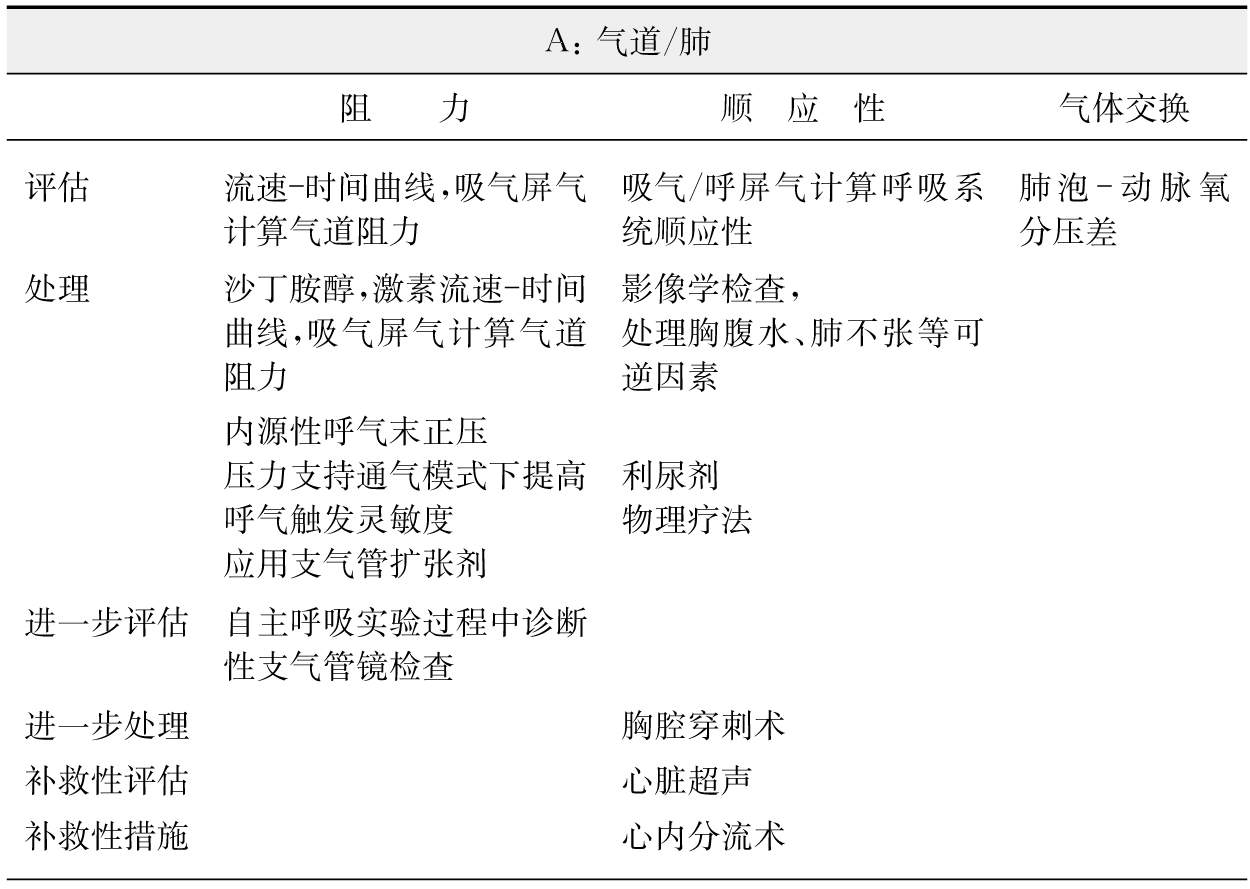
\includegraphics[width=\textwidth,height=\textheight,keepaspectratio]{./images/Image00082.jpg}\\
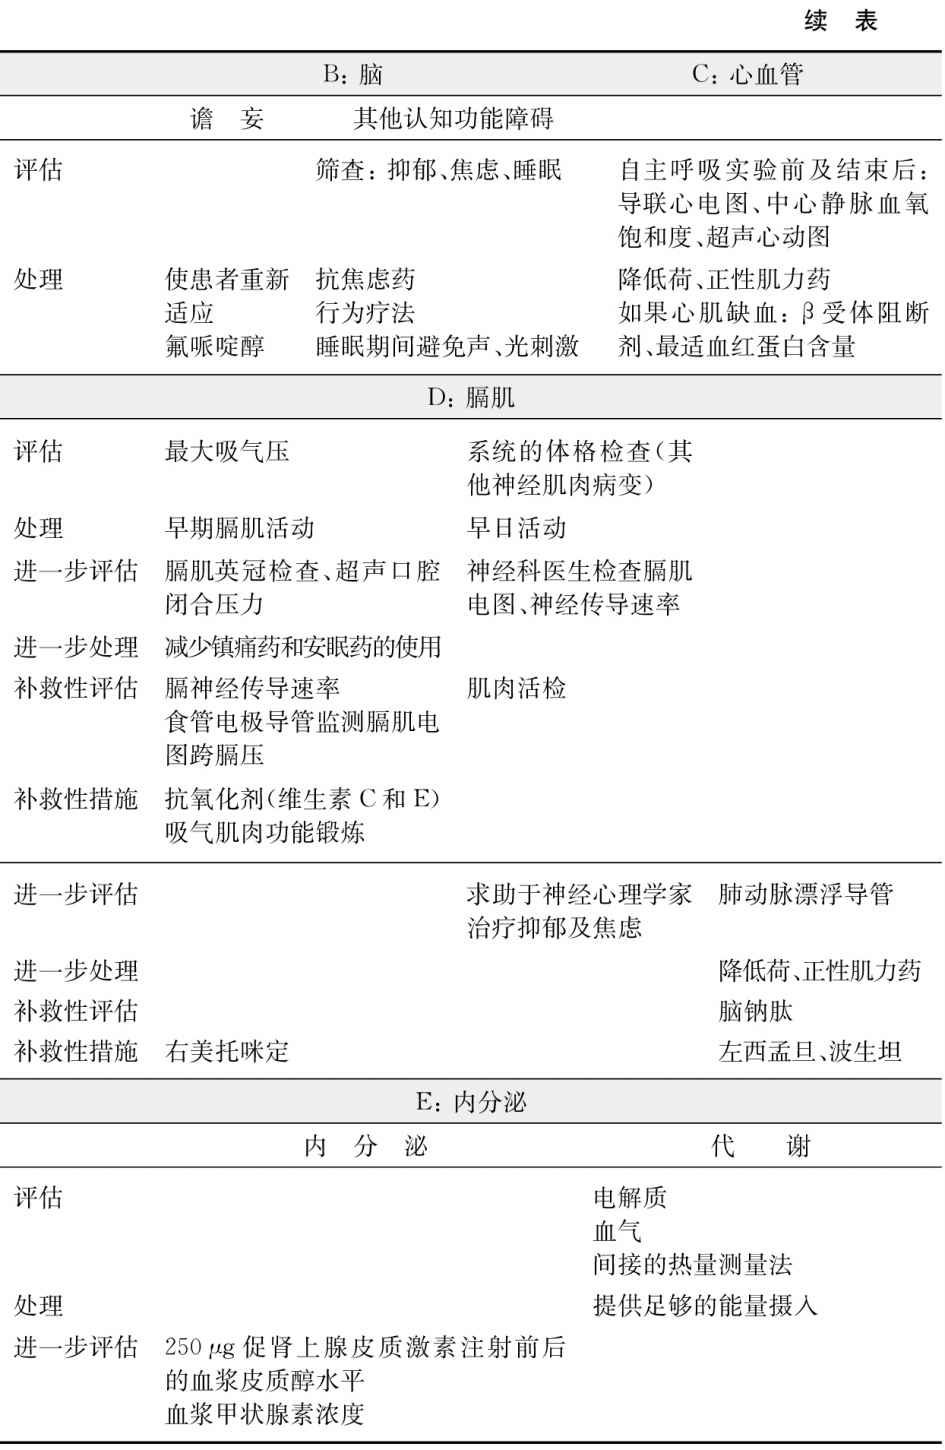
\includegraphics[width=\textwidth,height=\textheight,keepaspectratio]{./images/Image00083.jpg}
\end{longtable}

\subsubsection{哪些因素影响重症患者呼吸肌的做功能力?}

影响患者呼吸肌的做功能力的因素包括:

(1)呼吸中枢的兴奋性 呼吸中枢兴奋性降低,即呼吸中枢的传出冲动减少,导致呼吸肌做功能力下降。主要见于颅脑损伤引起的延髓呼吸中枢损害、高位脊髓损伤、膈神经损伤、吉兰-巴雷综合征等神经系统损害以及慢性阻塞性肺病导致的高二氧化碳抑制呼吸中枢等。在脱机困难中,呼吸中枢兴奋性降低是较少见的原因。

(2)呼吸肌收缩功能 呼吸肌收缩功能包括收缩强度和持久力,是决定患者是否能够脱机的主要因素。呼吸肌收缩功能降低主要见于肌肉疾病(重症肌无力、周期性麻痹等)、休克导致呼吸肌血供下降、严重营养不良、呼吸机过度支持导致的呼吸肌废用性萎缩、各种原因引起呼吸肌负荷过高导致呼吸肌疲劳、酸碱及电解质紊乱(酸中毒、低血钾等)及药物(肌松剂)对呼吸肌功能的抑制。

在治疗上应积极治疗原发病、纠正休克及酸碱平衡电解质紊乱、早期积极营养支持,同时应把握呼吸支持的水平,防止呼吸肌废用性萎缩。

\subsubsection{哪些因素可导致重症患者呼吸负荷明显增加?}

呼吸肌负荷增加是导致脱机困难最常见的原因。主要见于以下几个原因:

(1)呼吸系统本身因素导致的呼吸负荷增加 气道阻力增加、肺及胸廓顺应性降低及内源性呼气末正压是增加呼吸负荷的常见原因,可明显增加呼吸功。积极治疗原发性肺损害,改善肺的机械特征是十分重要的。

(2)气管插管或气管切开管及连接管的阻力过高 气管插管内径过细、插管腔内分泌物粘附或堵塞、插管过长及弯度过大均明显增加阻力,使呼吸肌需额外克服这部分阻力做功。6.5mm气管插管的阻力与正常气道阻力大致相等,而克服气管插管阻力所需的额外做功大约为正常呼吸功的20%~30%。这一点须引起临床重视。

(3)呼吸机及持续气道内正压系统的阻力过高 呼吸机阻力主要由管道阻力和按需活瓣灵敏度决定,正常情况下很低,但管理不当引起管道积水、管道扭曲、过滤器堵塞时,阻力明显增加。持续气道内正压系统气体流速不能满足患者吸气需要时,可引起患者呼吸功增加。加强呼吸机管理、使用高流量持续气道内正压系统可减少器械阻力。

\subsubsection{哪些指标可反映机械通气患者的呼吸中枢兴奋性?}

反映呼吸中枢兴奋性的指标包括:

(1)平均吸气流速 平均吸气流速是较好反映呼吸驱动的指标,但受肺机械特征影响较大,限制了其应用。

(2)口腔闭合压力(P\textsubscript{0.1}
) 口腔闭合压力为气道关闭时,吸气0.1秒钟时的口腔压力或胸腔内压力。测胸腔内压力较气道压力更为准确,它不受气道阻力等机械因素的影响,但受呼吸肌收缩功能的影响,口腔闭合压力与膈神经及膈肌肌电图的改变呈线性相关,是反映呼吸中枢兴奋性的常用手段。正常值为2~4cm
H\textsubscript{2}
O。口腔闭合压力增高见于:①呼吸肌机械负荷过重,呼吸中枢代偿性活动增强;②呼吸肌功能未完全恢复,产生一定收缩力需较大的中枢驱动。当口腔闭合压力>6cm
H\textsubscript{2} O时,脱机困难。

\subsubsection{哪些指标可反映机械通气患者的呼吸肌功能?}

反映呼吸肌功能的指标包括呼吸肌收缩强度指标和呼吸肌持久力指标。

呼吸肌收缩强度指标包括:

(1)最大吸气负压 是反映呼吸肌力量的指标,为最大吸气时,胸腔内或气道内压力的变化。正常值为>20cm
H\textsubscript{2} O。最大吸气压低于20cm H\textsubscript{2}
O说明呼吸肌收缩储备力下降,呼吸肌疲劳。大多数机械通气的患者最大吸气压低于40~50cm
H\textsubscript{2}
O,甚至其中一部分患者是呼吸机依赖者,因此,最大吸气压很难作为评价呼吸肌功能的可靠指标。

(2)肺活量 也是反映呼吸肌力量的指标,但测定肺活量需要患者的合作,这在重症医学科的重症患者常常难以做到。

反映呼吸肌持久力指标包括:

(1)机械力储备 每分通气量/最大每分通气量和潮气量/肺活量是反映呼吸肌功能储备的指标,用于评价和指导脱机、拔管。正常值均<50%。

(2)膈肌肌电图 膈肌电图高频波(50~100Hz)与低频波(0~25Hz)的比率是非特异性的反映呼吸肌疲劳的敏感指标。该方法需电极插入膈肌,为有创性,而非创伤性的体表膈肌电图可靠性差。

反映膈肌效能的指标为:

(1)神经机械效能 可反映膈肌的收缩效能。呼吸中枢发放冲动至膈神经,膈肌产生电兴奋后,通过电-机械耦连使膈肌收缩,胸腔内压下降。随着膈肌电活动的增加胸腔内负压也不断增加。但就不同患者而言,由于膈肌收缩能力不同,胸腔内负压随膈肌电活动增加的程度也不同,如能同时监测膈肌电活动及其产生的胸腔内压变化,计算单位膈肌电活动所产生胸腔内压即为神经机械效能(neuro-mechanical
efficiency,NME),可反映膈肌收缩效能。神经机械效能的测定是在呼气屏气的情况下,计算吸气时气道压力下降与对应的膈肌电活动比值,神经机械效能=压力下降/膈肌电活动。

(2)神经通气效能 反映呼吸中枢驱动下,膈肌产生通气的效能。在同一患者中,随着膈肌电活动增加,潮气量也明显增加。与正常人相比,慢性阻塞性肺疾病及脊髓前角灰质炎病人产生相同潮气量时的膈肌电活动明显增高。反之,就不同患者而言,由于其神经传导、膈肌功能及呼吸负荷不同,潮气量随膈肌电活动增加的程度也不同,潮气量与膈肌电活动密切相关。如能同时监测膈肌电活动及其产生潮气量,用潮气量除以膈肌电活动是神经通气效能最为简便的计算方法,当然比较神经机械效能更为准确的方法,是在确定的膈肌电活动下比较其产生潮气量的大小。神经机械效能的床边测定也非常简便。在没有额外呼吸支持的情况下(如持续气道内正压通气模式),同时记录膈肌电活动极其产生潮气量的大小,计算单位膈肌电活动产生的潮气量变化即可,神经机械效能=潮气量/膈肌电活动。其他指标:平均吸气压力、吸气时间占整个呼吸周期的百分比(Ti/Ttot)、平均吸气压力与最大吸气压力的百分比(P/Pmax)、压力-时间指数(PTI=P/PmaxX
Ti/Ttot)可用于判断呼吸肌的持久力。研究认为,当压力时间指数=0.40时,膈肌最大吸气压力百分比>40%或压力时间指数>0.15提示患者无力克服呼吸负荷,不能脱机。在临床上作为脱机的指标,需进一步研究和评价。

上述反映呼吸肌收缩强度和持久力的指标虽然有一定的临床价值,但采集资料常常很困难,在重症患者中使用往往受限。

\subsubsection{如何评价成比例辅助通气在机械通气撤机中的应用?}

比例辅助通气是采用正反馈原理,由呼吸机将患者吸气努力按预设比例放大的一种辅助通气模式。比例辅助通气可应用于撤机过程,当患者具备了撤机基本条件后,可逐步降低比例辅助通气辅助比例以增加患者做功比例,直至撤机。目前比例辅助通气辅助比例降至何种程度是撤机的合适标准尚无定论,有学者主张在患者具备撤机的基本条件后可先将比例辅助通气辅助比例设为70%,并根据患者呼吸及各项生理指标情况每1~2小时降低辅助比例10%~20%,指导辅助比例降至10%~20%或呼气末正压≤5cm
H\textsubscript{2} O时可考虑拔除气管插管。

由于比例辅助通气通气原理的特殊性,比例辅助通气与其他常用的撤机模式(如压力支持通气、同步间歇指令通气)相比,具有一定的优势
\protect\hyperlink{text00016.htmlux5cux23ch7-15}{\textsuperscript{{[}7{]}}}
:①比例辅助通气通气时,呼吸机与患者呼吸中枢的同步性更好。研究证实,压力支持通气及同步间歇指令正压通气通气时的呼气不同步往往导致无效触发或双触发等现象,呼吸频率明显受呼气不同步的影响。而比例辅助通气通气时,由于神经性吸气的结束即链接呼吸机送气的结束,不会出现呼气不同步现象,人机协调性更好,对及时撤机有利。②比例辅助通气通气呼吸机适应患者通气需求的能力更好。由于比例辅助通气是将患者呼吸努力放大的正反馈系统,因此,能随着患者呼吸努力的变化而改变支持的力度,能更好地适应患者通气需求的变化。研究证实,压力支持通气及比例辅助通气通气过程中,当束缚患者胸腹部致呼吸阻力增加,或急性二氧化碳潴留导致呼吸需求增加时,虽然此时压力支持通气通气患者呼吸肌做功明显高于比例辅助通气,但压力支持通气模式潮气量明显下降,主要通过增加呼吸频率来保证分钟通气量,而比例辅助通气模式潮气量下降及呼吸频率增加不明显。证实了与压力支持通气相比,比例辅助通气能更好的适应患者通气需求的变化。③镇静剂的用量减少。比例辅助通气患者舒适度高,人机对抗减少
\protect\hyperlink{text00016.htmlux5cux23ch5-15}{\textsuperscript{{[}5{]}}}
,也同时降低了因人机对抗导致的镇静剂用量。不适当的镇静往往导致撤机的延误,因此镇静剂的用量减少对及时撤机有利。④比例辅助通气可提高睡眠质量,良好的睡眠质量对撤机过程至关重要。睡眠时呼吸中枢兴奋性下降,呼吸频率的维持很大程度上依靠动脉血二氧化碳分压水平。如呼吸支持过度,可能会导致动脉血二氧化碳分压水平下降,患者呼吸中枢得不到有效刺激,导致呼吸暂停,待动脉血二氧化碳分压上升后才出现呼吸触发,并如此往复形成周期性呼吸暂停。睡眠中呼吸暂停可导致动脉血氧分压下降及睡眠中断,睡眠质量下降。研究显示,在压力支持通气及辅助控制模式通气时,患者夜间均会出现周期性呼吸暂停,而比例辅助通气时则无此现象。因此,理论上比例辅助通气应该是优于同步间歇指令正压通气及压力支持通气的一种撤机模式,但仍需要随机对照实验的证实。

\subsubsection{如何评价Smart care在呼吸机撤机中的地位?}

Smart
care是一种由机算计控制的自动化撤机系统。呼吸机可通过监测的潮气量、自主呼吸频率及呼气末二氧化碳分压水平自动尝试降低压力支持水平,直至压力支持水平降低到一定程度后患者呼吸仍稳定,呼吸机自动提示临床医师考虑撤机。近期的临床研究显示,150例患者随机分成传统撤机组(临床医师根据经验撤机)、撤机方案组和Smart
care撤机组,结果显示,与传统撤机组比较,Smart
care撤机组和撤机方案组能明显降低患者的机械通气时间、撤机时间(患者具备撤机条件到真正撤机的时间)、重症医学科住院时间及呼吸机相关性肺炎的发生率,但再插管率及住院病死率无显著差异。Lellouche等进行的多中心随机对照研究也显示,与应用本地方的传统撤机方案比较,Smart
care指导撤机能明显降低机械通气时间、撤机时间及重症医学科住院时间,同时再插管、气管切开及机械通气时间超过14或21天等并发症无显著差异。均提示Smart
care可能是一种更有效且安全的撤机方式。此外,由于Smart
care撤机过程由呼吸机自行控制,大大减轻了撤机过程中医生繁琐的工作,并使撤机步骤更加客观和程序化,是撤机方法的一大进步。

值得注意的是,Smart
care撤机过程仅依靠监测的呼吸参数来指导撤机,对患者其他脏器及全身情况缺乏全面的判断。因此,即使呼吸机提示撤机,最后是否撤机的决定也应由临床医师结合患者其他情况做出综合判断,不能完全依赖呼吸机,Smart
care起到的作用主要是提醒临床医师患者的呼吸功能已达到撤机标准。

\subsubsection{机械通气的患者符合哪些条件后应考虑进入撤机程序?}

导致机械通气的病因好转或去除后应开始进行撤机的筛查试验,筛查试验包括客观和主观评估两部分(表\ref{tab10-2}),具体内容包括下列4项:

\begin{table}[htbp]
\centering
\caption{撤机常用的筛查标准}
\label{tab10-2}
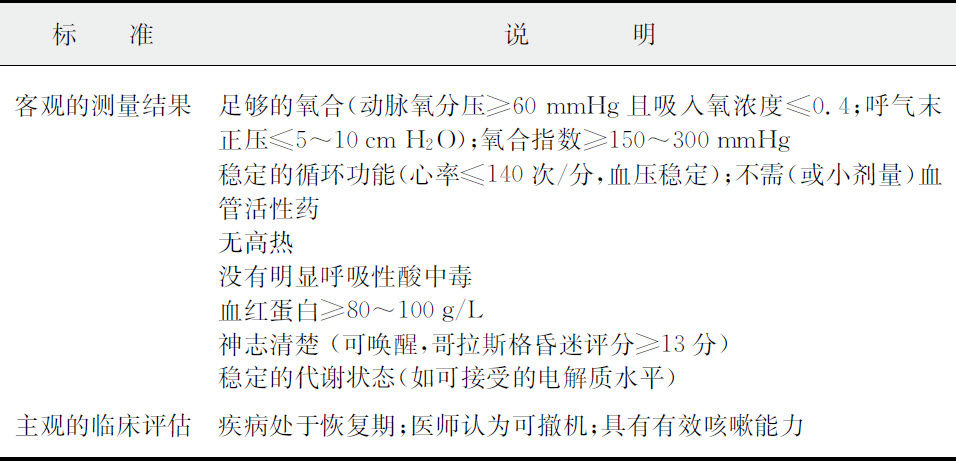
\includegraphics{./images/Image00084.jpg}
\end{table}

(1)导致机械通气的病因好转或去除;

(2)氧合指数>150~200mmHg;呼气末正压≤5~8cm H\textsubscript{2}
O;吸入氧浓度≤40%~50%;动脉血pH≥7.25;慢性阻塞性肺疾病患者动脉血pH>7.30,动脉血氧分压>50mmHg,吸入氧浓度<0.35;

(3)血流动力学稳定,没有心肌缺血动态变化,临床上没有显著的低血压,不需要血管活性药治疗或只需要小剂量血管活性药物如多巴胺或多巴酚丁胺每分钟<5~10μg/kg;

(4)有自主呼吸的能力。

医师的经验影响撤机的过程及结果,临床常发生过早撤机或延迟撤机,增加再插管率。可接受的再插管率应该在5%~15%之间。再插管使患者的院内获得性肺炎增加8倍,死亡风险增加6~12倍,而不必要延长机械通气可增加患者感染和其他并发症的风险,因此,尽早开始呼吸机撤机的筛查试验就显得很有必要。

\subsubsection{何谓自主呼吸试验?如何实施?}

自主呼吸试验(spontaneous breathing
trial,SBT)是临床上判断患者自主呼吸功能的有效方法。其基本方法是短期降低呼吸机支持水平或断开呼吸机后,观察患者自主呼吸情况及各项生理指标的变化,以对患者的自主呼吸能力做出判断,并为撤机提供参考。大量研究证实,SBT可为临床判断患者能否成功撤机提供信息,能耐受SBT的患者撤机成功率高,可考虑撤机。Esteban等对546名患者研究显示,有84%耐受SBT的患者撤机成功。其他研究也证实了能耐受SBT的患者撤机成功率在96%到77%之间
\protect\hyperlink{text00016.htmlux5cux23ch12-15}{\textsuperscript{{[}12{]}}}
。此外,SBT的实施非常安全,目前尚无数据显示SBT可直接导致任何的不良后果。因此,具备撤机条件的患者均应进行SBT。

SBT的实施可采用以下3种方式:①T管,直接断开呼吸机,并通过T管吸氧;②低水平持续气道内正压,将呼吸机调整至持续气道内正压模式,压力一般设为5cm
H\textsubscript{2}
O;③低水平的压力支持通气:将呼吸机调整至压力支持通气模式,支持压力一般设为5~7cm
H\textsubscript{2}
O。目前研究显示,采用上述3种方法进行SBT的效果基本一致,临床医师可结合患者具体情况选用SBT的方式。

\subsubsection{如何评估自主呼吸试验?}

符合筛查标准的患者并不一定能够成功的撤机,因此,需要对患者自主呼吸的能力做出进一步的判断,即自主呼吸试验(SBT)。目前较准确的预测撤机的方法是三分钟SBT,包括三分钟T管试验和持续气道内正压/压力支持通气试验。实施三分钟SBT时,应在患者床旁密切观察患者的生命体征,当患者出现超出下列指标时,应终止SBT,转为机械通气:①呼吸频率/潮气量(呼吸浅快指数)<105;②呼吸频率>8或<35次/分钟;③自主呼吸潮气量>4ml/kg;④心率应<140次/分或变化<20%,无新发的心律失常;⑤动脉血氧饱和度>90%。

三分钟SBT通过后,继续自主呼吸30~120分钟,如患者能够耐受可以确定撤机成功,可准备拔除气管插管。据文献报道,观察30分钟与120分钟的拔管成功率无差异,在SBT阶段进行监测评估,可以得到最有用的撤机信息以帮助临床决策。研究发现,通过SBT30~120分钟的患者至少有77%可以成功撤机
\protect\hyperlink{text00016.htmlux5cux23ch13-15}{\textsuperscript{{[}13{]}}}
\textsuperscript{,}
\protect\hyperlink{text00016.htmlux5cux23ch14-15}{\textsuperscript{{[}14{]}}}
。导致SBT失败的原因有多种,须注意的是气管插管引起的不适或持续气道内正压通气自动供气阀不敏感/触发不良等医源性因素。

\subsubsection{通过自主呼吸试验的患者是否就能立即拔除气管插管?}

通过自主呼吸试验的患者并不意味着就能成功拔除气管插管,决定拔除气管插管前还必须做气道的评估
\protect\hyperlink{text00016.htmlux5cux23ch15-15}{\textsuperscript{{[}15{]}}}
。拔管失败的原因与撤机失败的原因不同。上气道梗阻或患者气道保护能力差、气道分泌物清除能力不足,常常是拔管失败的原因。

(1)气道通畅程度的评价 机械通气时,把气管插管的气囊放气,可以用来评估上气道的开放程度(气囊漏气试验)。出现拔管后喘鸣的患者,可以使用类固醇和(或)肾上腺素,也可用无创通气和(或)氦氧混合气治疗,而不需重新插管。如果患者气囊漏气量较低,也可在拔管前24小时使用类固醇和(或)肾上腺素预防拔管后喘鸣。还应注意,气囊漏气量变低可能是由于分泌物在气管插管周围结痂形成外皮所致而非上气道水肿狭窄。在气囊漏气量低的患者拔管时,应将再插管的设备(包括气管切开设备)准备好。

(2)气道保护能力的评价 患者的气道保护能力对拔管成功是至关重要的。对患者的气道评估包括吸痰时咳嗽的力度、有无过多的分泌物和需要吸痰的频率(吸痰频率应>2小时/次或更长)。在神经肌肉病变和脊髓损伤的患者中,咳嗽时的峰流速>160L/分钟,预示可以拔管。

\subsubsection{自主呼吸试验失败的机械通气患者,应如何处理?}

自主呼吸试验(SBT)失败后应立即寻找原因。包括镇痛、镇静剂是否合理应用、血容量是否过多或不足、是否需要支气管扩张剂和存在心肌缺血等。

当SBT失败的原因纠正后每日进行一次SBT,没有必要一天内多次反复进行SBT。呼吸系统异常很少在数小时内恢复,一天内频繁的SBT对患者没有帮助。研究表明,SBT失败的原因常是呼吸系统机械力学的异常,而这些异常不能迅速恢复。

SBT失败后,机械通气应选择恒定的支持水平,以保证患者的呼吸肌充分休息,这可以大大缩短训练的时间。所以在SBT失败后的24小时,应该让肌肉休息、舒适(包括使用镇静剂)和避免并发症,而不是积极地降低通气支持的水平。

因此,若SBT失败,应给予充分的通气支持以缓解呼吸肌疲劳,并查找原因。

\subsubsection{何谓长期机械通气?应采取何种机械通气撤机策略?}

除非有明确的不可逆疾病的证据(例如,高位脊髓损伤或晚期的肌萎缩性脊髓侧索硬化),撤机失败3个月,为长期机械通气(permanent
mechanical ventilation,PMV)
\protect\hyperlink{text00016.htmlux5cux23ch11-15}{\textsuperscript{{[}11{]}}}
。

在20世纪80年代以前,这类患者长期在重症医学科中治疗,消耗了大量资源。对于长期机械通气患者,重症医学科不是适宜的治疗场所,应在医院内或医院外建立专门的撤机康复病房。部分长期机械通气的患者通过有计划的锻炼仍有撤机的希望,不能撤机的患者应制定终身的机械通气方案。

长期机械通气的患者很少采用每日自主呼吸试验,常使用辅助通气模式并逐步降低呼吸机条件以锻炼患者的呼吸肌。通常大约在通气支持条件降低到一半时,患者可转换到自主呼吸试验步骤。撤机锻炼的过程中,医务人员应留在患者身边,给予心理支持,并避免不必要的肌肉疲劳。

总的来说,长期机械通气患者应采用逐步降低机械通气水平和逐步延长自主呼吸时间的撤机策略。

\subsubsection{什么是序贯机械通气?}

机械通气患者撤机后常常需要无创通气进行序贯机械通气的辅助。序贯机械通气的目的主要在于缩短有创通气时间并辅助呼吸功能进一步恢复。无创、有创通气的根本区别在于呼吸机与患者的连接方式不同,无创通气以口/鼻面罩和患者相连,而有创通气需建立有创人工气道(气管插管或气管切开)。无创通气的应用使序贯通气的实施具有可操作性,并已经成功应用于一些类型的急性呼吸衰竭。随机对照的研究结果表明,慢性阻塞性肺病以及慢性呼吸衰竭基础上急性加剧的患者中,无创通气能显著缩短有创机械通气时间,减少并发症和死亡率。但是撤机失败导致的再插管延长插管时间,或者增加死亡率,通常这个过程并不能在应用无创通气后改善。因此,应慎重客观评估有创通气转变为无创通气的时机和指征。应用无创通气的患者一旦出现不能耐受或者病情反复应及时再插管
\protect\hyperlink{text00016.htmlux5cux23ch16-15}{\textsuperscript{{[}16{]}}}
。

\begin{center}\rule{0.5\linewidth}{\linethickness}\end{center}

参考文献

\protect\hyperlink{text00016.htmlux5cux23ch1-15-back}{{[}1{]}} .Slutsky
AS.Consensus conference on mechanical ventilation.Intensive Care
Med,1994,20:150-162.

\protect\hyperlink{text00016.htmlux5cux23ch2-15-back}{{[}2{]}} .Tobin
MJ.Advances in mechanical ventilation.N Engl J
Med,2001,344:1986-1996.

\protect\hyperlink{text00016.htmlux5cux23ch3-15-back}{{[}3{]}} .Pierson
DJ.Indications for mechanical ventilation in adults with acute
respiratory failure.Respir Care,2002,47:249-262.

\protect\hyperlink{text00016.htmlux5cux23ch4-15-back}{{[}4{]}}
.Dellinger RP,Carlet JM,Masur H,et al.Surviving sepsis campaign
guidelines for management of severe sepsis and septic shock.Intensive
Care Med,2004,30:536-555.

\protect\hyperlink{text00016.htmlux5cux23ch5-15-back}{{[}5{]}}
.Sevransky JE,Levy MM,Marini JJ.Mechanical ventilation in
sepsis-induced acute lung injury/acute respiratory distress syndrome:An
evidence-based review.Crit Care Med,2004,32:s548-s553.

\protect\hyperlink{text00016.htmlux5cux23ch6-15-back}{{[}6{]}} .Villar
J,Kacmarek RM,Perez-Mendez L,et al.A high positive end-expiratory
pressure,low tidal volume ventilatory strategy improves outcome in
persistent acute respiratory distress syndrome:a randomized,controlled
trial.Crit Care Med,2006,34:1311-1318.

\protect\hyperlink{text00016.htmlux5cux23ch7-15-back}{{[}7{]}} .Tassaux
D,Dalmas E,Gratadour P,et al.Patient-ventilator interactions during
partial ventilatory support:a preliminary study comparing the effects
of adaptive support ventilation with synchronized intermittent mandatory
ventilation plus inspiratory pressure support.Crit Care
Med,2002,30:801-807.

\protect\hyperlink{text00016.htmlux5cux23ch8-15-back}{{[}8{]}} .Kondili
E,Akoumianaki E,Alexopoulou C,et al.Identifying and relieving
asynchrony during mechanical ventilation.Expert Rev Respir
Med.2009;3:231-243.

\protect\hyperlink{text00016.htmlux5cux23ch9-15-back}{{[}9{]}}
.Piquilloud L,Vignaux L,Bialais E,et al.Neurally adjusted
ventilatory assist improves patient-ventilator interaction.Intensive
Care Med.2011;37:263-271.

\protect\hyperlink{text00016.htmlux5cux23ch10-15-back}{{[}10{]}} .Boles
JM,Bion J,Connors A,et al.Weaning from mechanical ventilation.Eur
Respir J,2007,29(5):1033-1056.

\protect\hyperlink{text00016.htmlux5cux23ch11-15-back}{{[}11{]}}
.Heunks LM,Hoeven JG.Clinical review:the ABC of weaning failure ---
a structured approach.Critical Care,2010,14:245.

\protect\hyperlink{text00016.htmlux5cux23ch12-15-back}{{[}12{]}}
.Esteban A,Alia I,Gordo F,et al.Extubation outcome after
spontaneous breathing trials with T-Tube or pressure support
ventilation.Am J Respir Crit Care Med,1997,156:459-465.

\protect\hyperlink{text00016.htmlux5cux23ch13-15-back}{{[}13{]}}
.Vallverdu I,Tobin MJ,Subiran M,et al.Clinical
characteristics,respiratory functional parameters,and outcome of a
two-hour T-piece trial in patients weaning from mechanical
ventilation.Am J Respir Crit Care Med,1998,158:1855-1862.

\protect\hyperlink{text00016.htmlux5cux23ch14-15-back}{{[}14{]}}
.Macintyre NR,Cook DJ,Ely EW,et al.Evidence-based guidelines for
weaning and discontinuing ventilatory
support.Chest,2001,120:375s-395s.

\protect\hyperlink{text00016.htmlux5cux23ch15-15-back}{{[}15{]}}
.Perren A,Domenighetti G,Mauri S,et al.Protocol-directed weaning
from mechanical ventilation:clinical outcome in patients randomized for
a 30-min or 120-min trial with pressure support ventilation.Intensive
Care Med,2002,28:1058-1063.

\protect\hyperlink{text00016.htmlux5cux23ch16-15-back}{{[}16{]}}
.Epstein,S.K.and C.G.Durbin,Jr.Should a patient be extubated and
placed on noninvasive ventilation after failing a spontaneous breathing
trial?Respiratory care,2010,55(2):198-206;discussion 207-208.

\protect\hypertarget{text00017.html}{}{}

